\documentclass[openany]{book}

\usepackage[a4paper,margin=4.72cm]{geometry}

\usepackage{graphicx}
\usepackage{wrapfig}
\usepackage{siunitx}
\usepackage[version=3]{mhchem}
\usepackage{natbib}
\usepackage{mathtools}
\usepackage{amssymb}
\usepackage{amsthm}
\usepackage[italian]{babel}
\usepackage{stackengine}
\usepackage{graphicx,ifthen}
\usepackage{amsmath}
\usepackage{hyperref}
\usepackage{upgreek}
\usepackage{bm}
\usepackage{braket}
\usepackage{float}
\usepackage{cancel}
\usepackage{anyfontsize}
\usepackage{scalefnt}

\newtheorem{lem}{Lemma}
\newtheorem{axiom}{Assioma}
\newtheorem{defn}{Definizione}
\newtheorem{obs}{Osservazione}
\newtheorem{ex}{Esempio}
\newtheorem{notz}{Notazione}
\newtheorem{corl}{Corollario}
\newtheorem{teo}{Teorema}
\theoremstyle{remark}
\newtheorem{caso}{Caso}

\numberwithin{lem}{chapter}
\numberwithin{axiom}{chapter}
\numberwithin{teo}{chapter}
\numberwithin{defn}{chapter}
\numberwithin{obs}{chapter}
\numberwithin{ex}{chapter}
\numberwithin{equation}{chapter}

\makeindex
\title{\textbf{APPUNTI DI \\ ESPERIMENTAZIONI II}}
\author{Manuel Gabriele Moretti}
\date{Agosto 2024}

\begin{document}

\maketitle
\pagenumbering{roman}
\tableofcontents
\newpage

\pagenumbering{arabic}

\chapter{Elettrotecnica}
La prima definizione fondamentale è quella dell'intensità di corrente.
\begin{defn}[intensità di corrente]
    \label{defn: intensità corrente}
    L'intensità di corrente è definita da
    \begin{equation}
        i(t)=\frac{dq}{dt},
    \end{equation}
    ovvero come la variazione di carica per unità di tempo.
\end{defn}
L'unità di misura della corrente è l'ampere [A]. Il verso della corrente $i$ in un circuito è opposto allo spostamento effettivo degli elettroni. Se la grandezza fisica dipende dal tempo si indica con la lettera minuscola. Il lavoro per spostare una carica attraverso una differenza di potenziale è
\begin{equation}
    dW=vdq=ivdt,
\end{equation}
quindi 
\begin{equation}
    \frac{dW}{dt}=iv.
\end{equation}
Segue in moto naturale la seguente definizione.
\begin{defn}[potenza]
    \label{defn:potenza}
    La potenza è definita da $p=iv$.
\end{defn}
L'unità di misura della potenza è il Watt [W]. La potenza può assumere due valori:
\begin{itemize}
    \item Se $p>0$, si dice che $p$ ha segno passivo, ovvero che l'elemento circuitale assorbe potenza.
    \item Se $p<0$, si dice che $p$ ha segno attivo, ovvero che l'elemento circuitale, emette potenza.
\end{itemize}
\begin{obs}
    Dato che il potenziale $v$ per convenzione parte sempre dal polo negativo verso quello positivo, $v$ è sempre positivo dato che viene calcolata come differenza tra il potenziale del polo positivo e di quello negativo. Dunque, se il verso della corrente $i$ e quello di $v$ sono opposti allora l'elemento assorbe potenza (come nel caso delle resistenze), invece se i versi sono concordi allora l'elemento genera potenza (come nel caso dei generatori).
\end{obs}
\begin{ex}
    Normalmente, la freccia che ruota indica la maglia, le frecce colorate rappresentano il potenziale degli elementi e le frecce nere rappresentano la direzione della corrente.
    \begin{figure}[h]
        \centering
        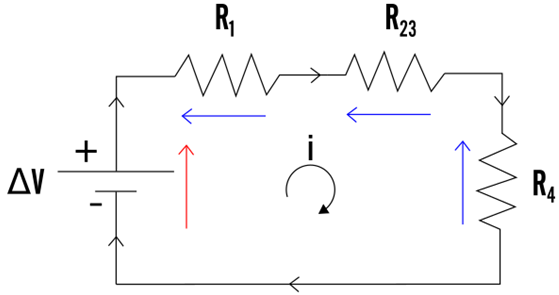
\includegraphics[width=0.5\linewidth]{Immagini/esempio circuito.png}
        \caption{esempio di diagramma circuitale.}
        \label{fig:esempio di circuito}
    \end{figure}
\end{ex}
Altre definizioni fondamentali per l'analisi di un circuito sono le seguenti.
\begin{defn}[nodo, ramo e maglia]\hfill
    \begin{enumerate} 
        \item Nodo: insieme di tre o più terminali uniti tra loro da connessioni ideali.
        \item Ramo: tratto del circuito che unisce due nodi.
        \item Maglia: percorso chiuso formato tra due rami del circuito che attraversa una sequenza di nodi senza passare più di una volta per uno stesso nodo e per uno stesso ramo.
    \end{enumerate}
\end{defn}
\begin{obs}
    Nel seguito, dato che si opera tramite modelli ideali della realtà, per semplicità si considera ogni tratto di filo con resistenza nulla.
\end{obs}

\section{Leggi di Ohm e di Kirchhoff}
\paragraph{Leggi di Ohm.} Le leggi di Ohm descrivono il comportamento di un resistore in un circuito elettrico attraversato da corrente.
\begin{axiom}[prima legge di Ohm]
    \label{ax:prima legge di ohm}
    La differenza di potenziale $V$ ai capi di un resistore è uguale al prodotto della resistenza $R$ per l'intensità di corrente $I$ che lo attraversa. In simboli,
    \begin{equation}
    \label{eq: VIR}
        V=IR.
    \end{equation}
\end{axiom}
L'unità di misura delle resistenza è l'Ohm [$\Omega$]. Se si provasse a misurare diversi valori della differenza di potenziale $\Delta V$ che attraversa il medesimo conduttore, si scoprirebbe che $\Delta V$ e $I$ sono legate da una relazione lineare. Tracciando un grafico di $\Delta V$ in funzione di $I$ si ottiene una retta passante per l'origine, il cui coefficiente angolare è proprio la resistenza. Quest'ultima osservazione corrisponde al fatto che a una corrente nulla corrisponde una differenza di potenziale nulla.
\begin{obs}
    La pendenza della retta $V=IR$ viene detta conduttanza e si indica con $G=1/R$. L'unità di misura della conduttanza è il Siemens [S].
\end{obs}
\begin{axiom}[seconda legge di Ohm]
    \label{ax: seconda legge di ohm}
    La resistenza di un conduttore è direttamente proporzionale alla sua lunghezza $l$, inversamente proporzionale alla sua sezione $A$ e dipende dal materiale di cui è costituito. In simboli
    \begin{equation}
        \label{eq: R=rl/A}
        R=\frac{\rho L}{A},
    \end{equation}
    dove $\rho$ è la resistività del conduttore, quantità che dipende unicamente dal materiale.
\end{axiom}
L'unità di misura della resistività è l'Ohm per metro [$\Omega\cdot m$]. Con sezione del conduttore si intende la sezione perpendicolare al moto delle cariche. 
\begin{obs}
    Se il materiale è isotropo allora la seconda legge di Ohm è valida nella forma dell'equazione \eqref{eq: R=rl/A}. Se questo non fosse il caso allora la resistività sarebbe una funzione della lunghezza del conduttore e la seconda legge di Ohm si dovrebbe riscrivere come 
    \begin{equation}
        R=\int_{a}^{b}\frac{\rho(L)}{A(L)}dL.
    \end{equation}
\end{obs}
\begin{obs}
    L'inverso della resistività è detto conduttività e si indica con $\sigma=1/\rho$. L'unità di misura della conduttività è il Siemens su metro [S/m].
\end{obs}
\paragraph{Leggi di Kirchhoff.} Le leggi di Kirchhoff sono due relazioni connesse con la conservazione della carica e dell'energia nei circuiti elettrici a parametri concentrati. Furono formulate da G. R. Kirchhoff nel 1845 a seguito di esperimenti empirici e precedono storicamente le ben più complesse e generali equazioni di Maxwell.
\begin{axiom}[prima legge di Kirchhoff]
    \label{ax:prima legge di kirchhoff}
    Definita una superficie chiusa che contenga un circuito elettrico in regime stazionario, la somma algebrica che attraversano la superficie (con segno diverso se entranti o uscenti) è nulla. Ovvero, in ogni istante di tempo si ha
    \begin{equation}
        \label{eq: sumI=0}
        \sum_{k=1}^{N}I_k=0.
    \end{equation}
\end{axiom}
\begin{ex}[applicazione prima legge di Kirchhoff]
    Considerando il circuito in figura \ref{fig:circuito I kirchhoff}, si può applicare la convenzione per i segni della corrente per entrambi i nodi del circuito a destra ottenendo il seguente sistema.
    \begin{equation}
        \begin{cases}
            I_1-I_2-I_3+I_4=0 \\
            -I_1+I_2+I_3-I_4=0.
        \end{cases}
    \end{equation}
    Si nota immediatamente che le due equazioni non sono indipendenti; infatti la seconda è equivalente alla prima a meno di un fattore moltiplicativo $(-1)$. È sufficiente pertanto un'unica equazione $I_1-I_2-I_3+I_4=0$.
        \begin{figure}[h]
        \centering
        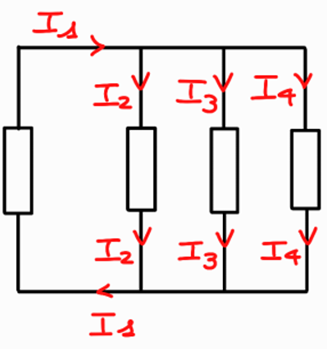
\includegraphics[width=0.25\linewidth]{Immagini/circuito I kirchhoff.png}
        \caption{circuito generico.}
        \label{fig:circuito I kirchhoff}
    \end{figure}
\end{ex}
    Si può quindi pensare come il numero di nodi indipendenti sia equivalente al numeri di nodi totali meno uno, ovvero
    \begin{equation}
        N_{indip}=N_{TOT}-1.
    \end{equation}
\begin{axiom}[seconda legge di Kirchhoff]
    \label{ax: seconda legge di kirchhoff}
    La somma algebrica delle tensioni agenti tra le coppie di punti nello spazio che formano una qualsiasi una sequenza chiusa (orientata) è uguale a zero. Più semplicemente, la somma algebrica delle tensioni lungo una linea chiusa (con il segno appropriato in funzione del verso di percorrenza della maglia stessa) è pari a zero. Ovvero in ogni istante di tempo si ha 
    \begin{equation}
        \label{eq: sumV=0}
        \sum_{k=1}^{N}V_k=0.
    \end{equation}
\end{axiom}
\begin{ex}[applicazione seconda legge di Kirchhoff]
    Considerando il circuito in figura \ref{fig:circuito II kirchhoff}, si può applicare la convenzione per i segni del potenziale ad ogni elemento circuitale ottenendo il seguente sistema.
    \begin{equation}
        \begin{cases}
            V_1-V_2-V_3=0 \\
            V_3-V_4-V_5=0 \\
            V_1-V_2-V_4-V_5=0.
        \end{cases}
    \end{equation}
    Si nota immediatamente come le tre equazioni non siano indipendenti; infatti, la terza è equivalente alla differenza tra la prima e la seconda. Sono sufficienti pertanto solo due equazioni
    \begin{equation}
        \begin{cases}
            V_1-V_2-V_3=0 \\
            V_3-V_4-V_5=0.
        \end{cases}
    \end{equation}
        \begin{figure}[H]
        \centering
        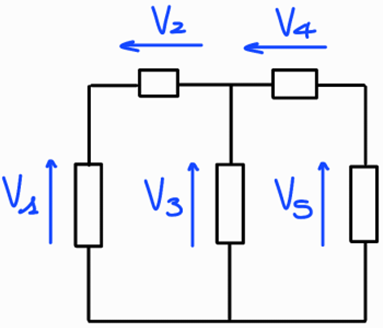
\includegraphics[width=0.25\linewidth]{Immagini/circuito II kirchhoff.png}
        \caption{circuito generico}
        \label{fig:circuito II kirchhoff}
    \end{figure}
\end{ex}
    In questo caso il ragionamento per ottenere il numero di maglie indipendenti non è diretto come per il caso dei nodi. Infatti, il numero di maglie indipendenti in un circuito è
    \begin{equation}
        M_{indip}=n_{rami}-N_{indip}=n_{rami}-N_{TOT}-1.
    \end{equation}

\subsection{Partitori} 
Si consideri in luogo il seguente circuito, detto partitore di tensione.
\begin{figure}[h]
    \centering
    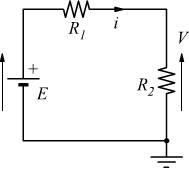
\includegraphics[width=0.37\linewidth]{Immagini/partitore di tensione.png}
    \caption{partitore di tensione.}
    \label{fig: partitore tensione}
\end{figure}
\begin{defn}[resistenze in serie]
    \label{defn: resistenze in serie}
    Due o più resistenze si dicono collegate in serie se sono attraversate dalla stessa corrente.
\end{defn}
Applicando la prima legge di Ohm ai due resistori si trovano
\begin{equation}
\label{eq: sistema partitore tensione}
    \begin{cases}
        V_1=IR_1 \\
        V_2=IR_2.
    \end{cases}
\end{equation}
Dall'equazione \eqref{eq: sumV=0} si trova invece che 
\begin{equation}
    \label{eq: V partitore tensione}
    V=V_1+V_2.
\end{equation}
Sommando pertanto le due equazioni del sistema \eqref{eq: sistema partitore tensione} si trova
\begin{equation}
    \label{eq: corrente partitore tensione}
    I=\frac{V}{R_1+R_2}.
\end{equation}
Sostituendo infine l'equazione \eqref{eq: corrente partitore tensione} nelle equazioni del sistema \eqref{eq: sistema partitore tensione} si trovano
\begin{equation}
    \label{eq: equazioni partitore tensione}
    \begin{cases}
        V_1=V\dfrac{R_1}{R_1+R_2} \\[2ex]
        V_2 = V\dfrac{R_2}{R_1+R_2}.
    \end{cases}
\end{equation}
Si nota quindi come il potenziale si ripartisce in funzione del potenziale totale e del valore delle resistenze. Inoltre, dall'equazione \eqref{eq: V partitore tensione} si deduce che per un qualsiasi numero di resistenze in serie vale
\begin{equation}
    \label{eq:resistenza equivalente serie}
    R_{eq}=R_1+\cdots+R_n=\sum_{i=1}^{n}R_i.
\end{equation}
Si consideri in luogo il seguente circuito, detto partitore di corrente.
\begin{figure}[H]
    \centering
    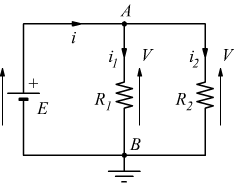
\includegraphics[width=0.4\linewidth]{Immagini/partitore di corrente.png}
    \caption{partitore di corrente.}
    \label{fig: partitore corrente}
\end{figure}
\begin{defn}[resistenze in parallelo]
    \label{defn: resistenze in parallelo}
    Due o più resistenze si dicono in parallelo quando ai capi di ciascuna di esse c'è la stessa differenza di potenziale.
\end{defn}
Applicando la prima legge di Ohm ai due resistori si trovano
\begin{equation}
    \label{eq: sistema partitore corrente}
    \begin{cases}
        V=I_1R_1 \\
        V=I_2R_2.
    \end{cases}
\end{equation}
Dall'equazione \eqref{eq: sumI=0} si trova invece che
\begin{equation}
    \label{eq: corrente partitore corrente}
    I=I_1+I_2.
\end{equation}
Risolvendo per $I_1$ e $I_2$ le equazioni del sistema \eqref{eq: sistema partitore corrente} si trova
\begin{equation}
    \label{eq: V partitore corrente}
    I=V\left(\frac{R_1+R_2}{R_1R_2}\right)\quad\therefore\quad V=\frac{IR_1R_2}{R_1+R_2}.
\end{equation}
Sostituendo nell'equazione \eqref{eq: V partitore corrente} le relazioni del sistema \eqref{eq: sistema partitore corrente} rispettivamente si trovano
\begin{equation}
    \label{eq: equazioni partitore corrente}
    \begin{cases}
        I_1=I\dfrac{R_2}{R_1+R_2} \\[2ex]
        I_2=I\dfrac{R_1}{R_1+R_2}.
    \end{cases}
\end{equation}
Si nota quindi come la corrente di ripartisce in funzione della corrente totale e del valore delle resistenze. Inoltre, dall'equazione \eqref{eq: corrente partitore corrente} si deduce che per un qualsiasi numero di resistenze in parallelo vale
\begin{equation}
    \label{eq: resistenze equivalente parallelo}
    R_{eq}=\left(\frac{1}{R_1}+\cdots+\frac{1}{R_n}\right)^{-1}=\left(\sum_{i=1}^{n}\frac{1}{R_i}\right)^{-1}.
\end{equation}

\subsection{Generatori reali}
In generale, in un circuito la circuitazione definita tramite la prima legge di Maxwell è diversa da zero, ossia
\begin{equation}
    \oint_{\gamma}\bm{E}\cdot d\bm{l}\neq0.
\end{equation}
Quindi il generatore di tensione sfrutta un processo non conservativo per generare una differenza di potenziale. In caso contrario, la circuitazione sarebbe nulla dato che il campo elettrostatico è conservativo.
\begin{obs}
    Tramite una cella elettrochimica è possibile creare una differenza di potenziale.
    \begin{figure}[h]
        \centering
        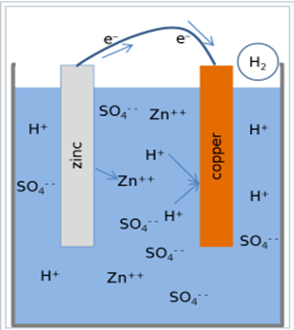
\includegraphics[width=0.3\linewidth]{Immagini/cella.png}
        \caption{cella elettrochimica.}
        \label{fig: cella elettrochimica}
    \end{figure}

Quando la cella fornisce una corrente elettrica al circuito esterno, lo zinco metallico sulla superficie dell'elettrodo di zinco si dissolve nella soluzione. Gli atomi di zinco si dissolvono nell'elettrolita liquido come ioni carichi elettricamente \ce{Zn^2+}, lasciando nel metallo due elettroni, secondo la reazione di ossidazione
\begin{equation}
        \ce{Zn -> Zn^2+ + 2e-}.
\end{equation}
Nel momento in cui lo zinco entra nell'elettrolita, due ioni idrogeno caricati positivamente dall'elettrolita $\ce{H+}$. Questi si combinano con due elettroni sulla superficie dell'elettrodo di rame e formano una molecola di idrogeno $\ce{H_2}$ priva di carica, secondo la reazione di riduzione
\begin{equation}
    \ce{ 2H+ + 2e- -> H_2}
\end{equation}
Gli elettroni utilizzati nel rame per formare le molecole di idrogeno vengono recuperati trasferendoli dallo zinco tramite un conduttore esterno che si collega tra rame e zinco. Le molecole di idrogeno formatesi sulla superficie del rame si disperdono sotto forma di idrogeno gassoso. 

Questa reazione è di tipo elettrochimico, dunque non è conservativa, lo zinco non si può ossidare all'infinito e, a meno che non si inverta il processo chimico. In particolare, la reazione termina naturalmente quando lo zinco caricatosi negativamente, respinge gli ioni $\ce{SO4^2-}$.

In sostanza, gli ioni $\ce{SO4^2-}$ e $\ce{H+}$ fungono da resistenza. Quindi, il modello di un generatore di tensione reale deve comprendere una resistenza interna allo stesso.
\end{obs}
\begin{defn}[generatore di tensione reale]
    Un generatore di tensione reale è tale se la differenza di potenziale che è in grado di mantenere ai suoi capi non coincide con la sua forza elettromotrice.
\end{defn}
\begin{figure}[h]
    \centering
    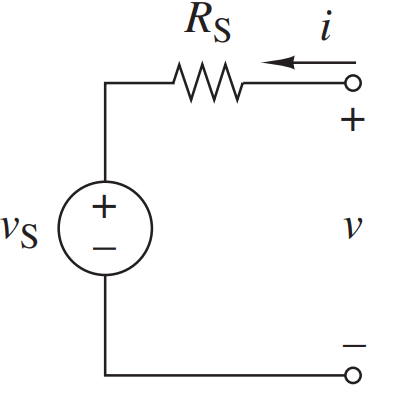
\includegraphics[width=0.3\linewidth]{Immagini/generatore tensione reale.png}
    \caption{generatore di tensione ideale.}
    \label{fig:generatore tensione reale}
\end{figure}

Considerando un circuito costituito da un generatore di tensione reale e un resistore, come quello in figura \ref{fig: circuito gen. tens. reale} si può ottenere la corrente erogata dal generatore e la differenza di potenziale ai capi di esso. Applicando la prima legge di Ohm alle due resistenze si ottiene
\begin{equation}
\label{eq: sistema gen. tens. reale}
    \begin{cases}
        \Delta V_R=RI \\
        \Delta V_r=rI
    \end{cases}.
\end{equation}
Usando ora l'equazione \eqref{eq: sumV=0} si ha che
\begin{equation}
    fem-\Delta V_r-\Delta V_R=0,
\end{equation}
da cui, sostituendo le equazioni del sistema \eqref{eq: sistema gen. tens. reale}, si trova la corrente $I$ erogata dal generatore
\begin{equation}
    \label{eq: corrente gen. tens. reale}
    I=\frac{fem}{r+R}.
\end{equation}
Ora, dato che $\Delta V=RI$, si trova la differenza di potenziale del generatore
\begin{equation}
    \label{eq: V gen. tens. reale}
    \Delta V=\frac{R}{r+R}fem.
\end{equation}
\begin{figure}[h]
    \centering
    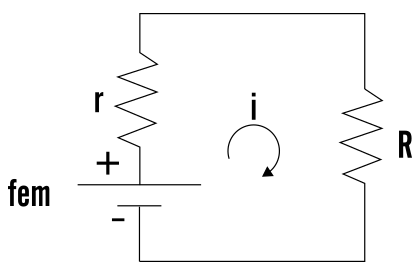
\includegraphics[width=0.4\linewidth]{Immagini/esempio circuito gen. tens. reale.png}
    \caption{circuito con un generatore reale di tensione.}
    \label{fig: circuito gen. tens. reale}
\end{figure}
\begin{defn}[generatore di corrente reale]
    Un generatore di corrente reale è tale se la corrente erogata non coincide con la corrente erogata dal generatore ideale corrispondente.
\end{defn}
\begin{figure}[h]
    \centering
    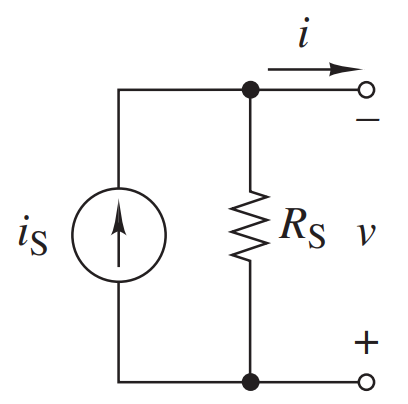
\includegraphics[width=0.3\linewidth]{Immagini/generatore corrente reale.png}
    \caption{generatore di corrente reale.}
    \label{fig:gen. corr. reale}
\end{figure}
\begin{teo}[teorema del generatore equivalente]
    \label{teo: gen. equivalente}
    Un generatore di tensione reale può essere convertito in un generatore di corrente reale, e viceversa.
\end{teo}
Infatti, considerando la figura \ref{fig:generatore tensione reale}, per la seconda legge di Ohm si ha $V_S=IR_S$ da cui
\begin{equation}
    I=\frac{V_S}{R_S}.
\end{equation}
\begin{figure}[ht]
    \centering
    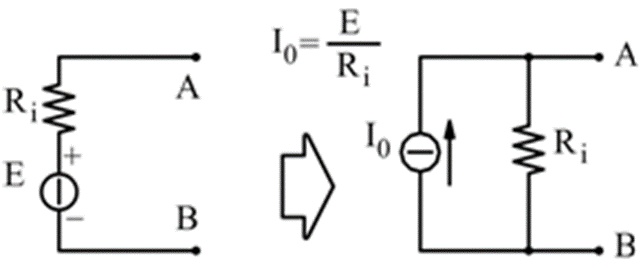
\includegraphics[width=0.5\linewidth]{Immagini/teorema del generatore equivalente.png}
    \caption{conversione di un generatore di tensione reale.}
    \label{fig: conversione gen. tens. reale}
\end{figure}

\section{Strumenti di misura}
\paragraph{Amperometro.} L'amperometro ideale è un bipolo la cui resistenza è nulla e che misura la corrente che passa in un ramo di un circuito. Essendo a resistenza nulla la sua inserzione in serie a qualsiasi ramo del circuito non altera in alcun modo il funzionamento del circuito medesimo; l'amperometro ideale si comporta infatti come un cortocircuito.
\begin{figure}[h]
    \centering
    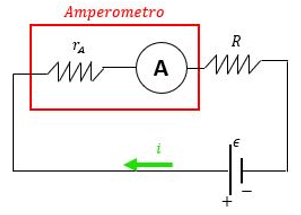
\includegraphics[width=0.35\linewidth]{Immagini/amperometro.png}
    \caption{circuito con amperometro.}
    \label{fig:circuito con amperometro}
\end{figure}

L'amperometro quindi restituisce il valore della corrente che lo attraversa. Chiaramente, poiché non esistono nella realtà amperometri con resistenza nulla, il valore della corrente che ci restituisce l'amperometro non è esattamente uguale a quello della corrente che circola nel circuito in assenza dell'amperometro. Quest'ultima corrente è
\begin{equation}
    I=\frac{E}{R}.
\end{equation}
Con l'amperometro nel circuito si aggiunge in serie la resistenza $R_a$, ottenendo
\begin{equation}
    I'=\frac{E}{R+R_a}.
\end{equation}
Chiaramente, $I'<I$. Questo effetto è detto ``effetto di carico''. Per rendere la differenza tra $I'$ e $I$ minima si deve avere $R_a\ll R$.

\paragraph{Voltmetro.} Il voltmetro ideale è un bipolo la cui resistenza è infinita, equivale quindi ad un circuito aperto. Essendo a resistenza infinita la sua inserzione tra due punti di un circuito non altera in alcun modo il funzionamento del circuito medesimo. Malgrado, ovviamente, non esistano nella realtà voltmetri ideali, ha una notevole importanza teorica e nella simulazione dei circuiti.
\begin{figure}[h]
    \centering
    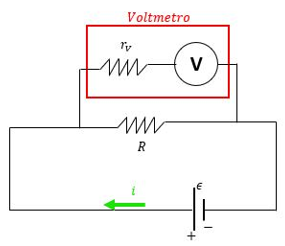
\includegraphics[width=0.37\linewidth]{Immagini/voltmetro.png}
    \caption{circuito con voltmetro.}
    \label{fig:circuito con voltmetro}
\end{figure}

Il voltmetro restituisce la differenza di potenziale tra due punti del circuito. Chiaramente, poiché non esistono nella realtà voltmetri con resistenza infinita, la differenza di potenziale che restituisce il voltmetro non è esattamente uguale a quello della differenza di potenziale che è presente in assenza di esso. Quest'ultima differenza di potenziale in assenza del voltmetro è
\begin{equation}
    V=\frac{ER}{R_i+R}.
\end{equation}
Con il voltmetro nel circuito si aggiunge in parallelo la resistenza $R_v$ del voltmetro, ottenendo
\begin{equation}
    V'=\frac{ER_{eq}}{R_i+R_{eq}},\quad R_{eq}=\frac{R\cdot R_v}{R+R_v}.
\end{equation}
Chiaramente, $V'<V$. Questo effetto è detto ``effetto di carico''. Per rendere la differenza tra $V'$ e $V$ minima si deve avere $R_v\approx R$.

\paragraph{Galvanometro.} Gli amperometri magnetoelettrici misurano la corrente attraverso una misurazione indiretta del campo magnetico generato da essa. Il galvanometro di Deprez-d'Arsonval è stato il primo tipo di amperometro magnetoelettrico.
\begin{figure}[h]
    \centering
    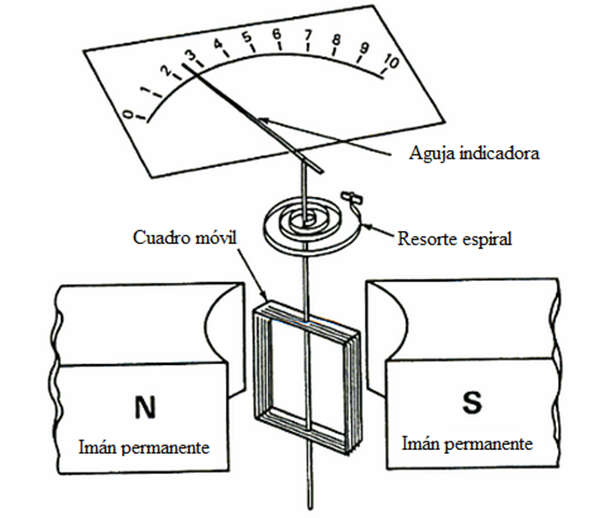
\includegraphics[width=0.5\linewidth]{Immagini/galvanometro.png}
    \caption{diagramma di un galvanometro.}
    \label{fig: galvanometro}
\end{figure}

L'espressione matematica della forza di un campo magnetico su un filo percorso da corrente è data dalla seconda legge di Laplace $d\bm{F}=i\cdot d\bm{l}\times \bm{B}$. Quindi, la forza totale subita dal quadro mobile in modulo è 
\begin{equation}
    F=ibBN,
\end{equation}
dove $N$ è il numero di spire del quadro. Il momento della forza $\bm{F}$ è
\begin{equation}
    M_e=hF=IbBNh=K_MI.
\end{equation}
Chiaramente il quadro in questa situazione continuerebbe a girare, l'obiettivo è però misurare il valore della corrente $I$. Consideriamo quindi il momento $M_r$ causato dalla forza di richiamo della spirale, la quale funge da molla, dato da
\begin{equation}
    M_r=K_r\theta,
\end{equation}
dove $\theta$ è l'angolo creato dalla lancetta del galvanometro. Nella situazione di equilibrio si ha quindi 
\begin{equation}
    M_r=M_e\quad\Rightarrow\quad K_r\theta=K_MI,
\end{equation}
da cui
\begin{equation}
    \label{eq: corrente galvanometro}
    I=\frac{K_r}{K_M}\theta=\mathcal{K}\theta.
\end{equation}

\paragraph{Galvanometro come voltmetro.} Per aumentare la portata di potenziale misurabile con il galvanometro si deve aggiungere una resistenza in serie del voltmetro $R_{SV}$ tale che
\begin{equation}
    \frac{V_{FS}}{R_{SV}+R_G}=I_{FSG},
\end{equation}
dove $V_{FS}$ è la differenza di fondo scala, ovvero la massima misurabile, e $1/I_{FSG}$ è la sensibilità del galvanometro.

\paragraph{Galvanometro come amperometro.} Per aumentare la portata di corrente del galvanometro invece si deve aggiungere una resistenza in parallelo a quest'ultimo. Inoltre, poiché la differenza di potenziale ai capi delle due resistenze è la stessa,
\begin{equation}
    I_GR_G=I_{sh}R_{sh}\quad\therefore\quad I=I_G\left(1+\frac{R_G}{R_{sh}}\right)=I_GK
\end{equation}
dove $R_{sh}$ è detta resistenza di shunt e $K$ è detto fattore di amplificazione.

\paragraph{Galvanometro come ohmetro.} Il galvanometro può essere usato per determinare il valore di una resistenza ignota. In questo caso non è possibile sfruttare la corrente del circuito ma è necessaria una batteria esterna. Considerando il circuito in figura \ref{fig: galv. ohm.} si ha che:
\begin{enumerate}
    \item nel caso $R_x=0$, allora
    \begin{equation}
        I_{FSG}=\frac{V_S}{R_S+R_S+R_T};
    \end{equation}
    \item nel caso $R_x\to\infty$, allora 
    \begin{equation}
        0=\frac{V_S}{R_S+R_S+R_T+R_x}.
    \end{equation}
\end{enumerate}
\begin{figure}[h]
    \centering
    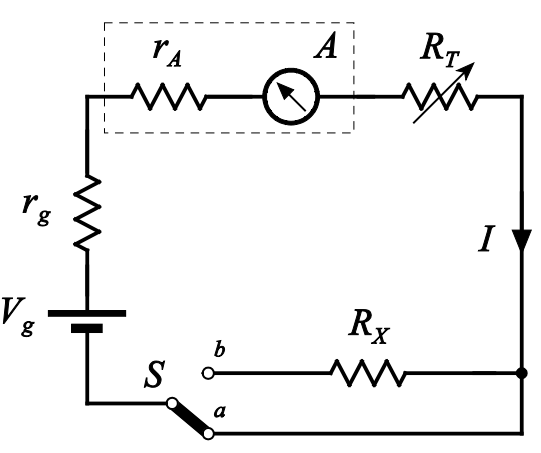
\includegraphics[width=0.4\linewidth]{Immagini/galv. ohmetro.png}
    \caption{circuito con galvanometro come ohmetro.}
    \label{fig: galv. ohm.}
\end{figure}

\section{Analisi delle maglie e dei nodi}

\paragraph{Analisi delle maglie.}Un metodo utile per risolvere un gran numero di circuiti è il metodo delle maglie, detto anche analisi delle maglie. Il metodo si basa sulle maglie indipendenti di un circuito e delle leggi di Kirchhoff. 
\begin{ex}
    Si consideri il seguente circuito.
    \begin{figure}[h]
        \centering
        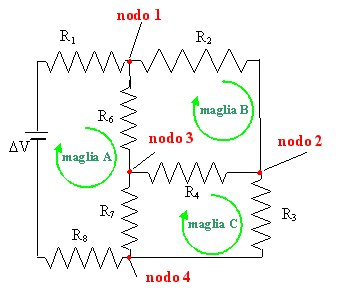
\includegraphics[width=0.5\linewidth]{Immagini/circuito analisi maglie.png}
        \caption{esempio di circuito risolvibile con il metodo della maglie.}
        \label{fig: circuito maglie}
    \end{figure}
    
    Si comincia individuando le maglie indipendenti del circuito. Queste possono essere facilmente individuate pensando ad esse come le "finestre" del circuito. In questo caso quindi sono tre. Ricordando ora le leggi di Kirchhoff si ottiene il seguente sistema.
    \begin{equation}
        \begin{cases}
            (R_1+R_6+R_7+R_8)I_{mA}-R_6I_{mB}-R_7I_{mC}=\Delta V \\
            -R_6I_{mA}+(R_6+R_2+R_4)I_{mB}-R_4I_{mC}=0 \\
            -R_7I_{mA}-R_4I_{mB}+(R_7+R_3+R_4)I_{mC}=0.
        \end{cases}
    \end{equation}
\end{ex}
Da qui è possibile poi ricavare le incognite del circuito a seconda dei dati noti.

\paragraph{Analisi dei nodi.} Un altro metodo utile per risolvere un gran numero di circuiti, molto simile al precedente, è il metodo dei nodi, detto anche analisi dei nodi. Il metodo si basa sulle leggi di Kirchhoff e sulla scelta di un potenziale di riferimento arbitrario, di solito la terra. 
\begin{ex}
    Si consideri il circuito in figura \ref{fig: circuito nodi}. Si comincia con scegliere come nodo di riferimento il primo nodo in basso, assegnandoli potenziale nullo $V_0=0$. Ai restanti due nodi si assegna potenziale $V_2$ e $V_1$ (a sinistra e a destra della resistenza di 4$\Omega$ rispettivamente). Si assegna quindi la corrente ad ogni ramo, $I_k$, con $k=1,\dots,5$. In questo caso, $I_1=5$ A e $I_4=10$ A. Usando l'equazione \eqref{eq: sumI=0}, sui nodi 1 e 2 si hanno rispettivamente
    \begin{equation}
        \label{eq: corrente nodo 1}
        I_4+I_2=I_1+I_5,
    \end{equation}
    \begin{equation}
        \label{eq: corrente nodo 2}
        I_1=I_2+I_3.
    \end{equation}
    Ora, con la seconda legge di Ohm, si riscrivono le equazioni delle correnti $I_2$, $I_3$ e $I_5$, ottenendo
    \begin{equation}
        \begin{cases}
            I_2=\dfrac{V_2-V_1}{4} \\[2ex]
            I_3=\dfrac{V_2-V_0}{2}=\dfrac{V_2}{2} \\[2ex]
            I_4=\dfrac{V_1-V_0}{6}=\dfrac{V_1}{6}.
        \end{cases}
    \end{equation}
    Ora sostituendo queste nelle equazioni \eqref{eq: corrente nodo 1} e \eqref{eq: corrente nodo 2} si trovano $V_1=20$ e $V_2=40/3$. Da cui si possono semplicemente ricavare le correnti.
    \begin{figure}[h]
        \centering
        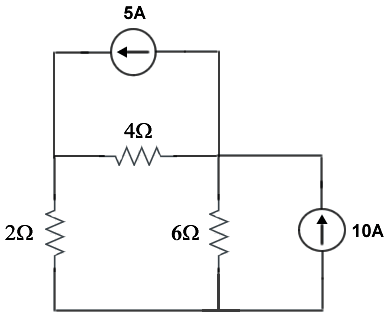
\includegraphics[width=0.35\linewidth]{Immagini/circuito analisi nodi.png}
        \caption{esempio di circuito risolvibile con il metodo dei nodi.}
        \label{fig: circuito nodi}
    \end{figure}
\end{ex}

\paragraph{Sistema ponte.} Un sistema ponte è un circuito del tipo rappresentato in figura \ref{fig: sistema ponte}. Le resistenze del circuito non possono essere semplificate poiché queste non sono né in parallelo né in serie. Invece, è possibile usare l'analisi dei nodi per risolvere il circuito. In questo caso si ottiene
\begin{equation}
    \begin{cases}
        \left(\dfrac{1}{R_1}+\dfrac{1}{R_2}+\dfrac{1}{R_3}\right)V_A-\dfrac{1}{R_1}V_B-\dfrac{1}{R_2}V_C=\dfrac{E}{R} \\[2ex]
        \left(\dfrac{1}{R_1}+\dfrac{1}{R_3}+\dfrac{1}{R_5}\right)V_B-\dfrac{1}{R_5}V_C-\dfrac{1}{R_1}V_A=0 \\[2ex]
        \left(\dfrac{1}{R_2}+\dfrac{1}{R_4}+\dfrac{1}{R_5}\right)V_C-\dfrac{1}{R_2}V_A-\dfrac{1}{R_5}V_B=0
    \end{cases}
\end{equation}
\begin{figure}[h]
    \centering
    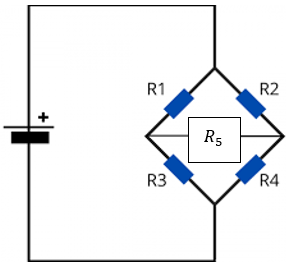
\includegraphics[width=0.29\linewidth]{Immagini/sistema ponte.png}
    \caption{sistema ponte.}
    \label{fig: sistema ponte}
\end{figure}

Inoltre, se $V_B=V_C$ allora il ponte si dice bilanciato. In questo caso la resistenza $R_5$ può essere eliminata riducendo il circuito a due coppie di resistenze in parallelo, che possono essere a loro volta risolte in un'unica resistenza.

\section{Teoremi per circuiti lineari}
\paragraph{Principio di sovrapposizione degli effetti.} Un principio fondamentale per la trattazione di circuiti lineari sul quale agiscono più ingressi è il teorema di sovrapposizione degli effetti. L'idea è quella di studiare lo stesso sistema più volte considerando un ingresso per volta ed annullando i rimanenti. Nella pratica, il generatore viene sostituito con un circuito chiuso, mentre quello di corrente con un circuito aperto. 
\begin{axiom}[principio di sovrapposizione degli effetti]
    La risposta di una rete lineare alla sollecitazione di più generatori indipendenti può essere ottenuta considerando ciascun generatore separatamente attivo e sommando algebricamente le rispettive risposte della rete.
\end{axiom}
\begin{ex}
    Si consideri il seguente circuito.
    \begin{figure}[h]
        \centering
        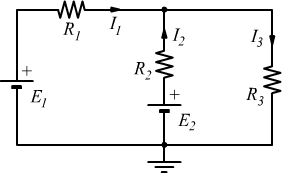
\includegraphics[width=0.4\linewidth]{Immagini/circuito PSE.png}
        \caption{circuito risolvibile con il principio di sovrapposizione degli effetti.}
        \label{fig: circuito PSE}
    \end{figure}

    Si può dapprima considerare agente solo $E_1$ cortocircuitando $E_2$ e si determinano le correnti parziali nei vari rami. Poi si considera agente solo $E_2$ cortocircuitando $E_1$ e si determinano le corrente parziali corrispondenti nei vari rami. In ciascun ramo la corrente effettiva è data dalla somma algebrica delle correnti parziali trovate separatamente, quindi
    \begin{equation}
        \begin{cases}
            I_1=I_1'+I_1'' \\
            I_2=I_2'+I_2'' \\
            I_3=I_3'+I_3''
        \end{cases}.
    \end{equation}
    Se una corrente risulta negativa significa solo che la vera corrente circolante ha il modulo uguale a quella trovata ma il senso di percorrenza reale è contrario a quello che inizialmente avevamo prefissato arbitrariamente.
\end{ex}

\paragraph{Teorema di Thevenin.} Un altro teorema fondamentale per la risoluzione di circuiti lineari è il teorema di Thevenin, con il quale è possibile semplificare circuiti anche molto complessi.
\begin{teo}[teorema di Thevenin]
    \label{teo: thevenin}
    Qualunque circuito lineare, indipendentemente dalla sua complessità, visto da due terminali è equivalente ad un generatore reale di tensione costituito da un generatore ideale in serie a un resistore.
\end{teo}
\begin{ex}
    Nel circuito seguente si vuole semplificare la parte evidenziata secondo il teorema \ref{teo: thevenin}.
    \begin{figure}[h]
        \centering
        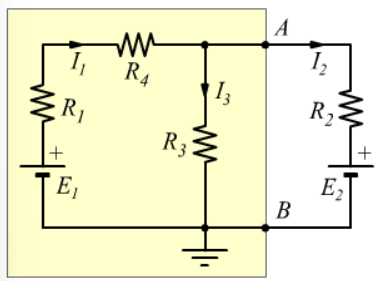
\includegraphics[width=0.4\linewidth]{Immagini/circuito thevenin.png}
        \caption{circuito risolvibile con il teorema di Thevenin.}
        \label{fig: circuito thevenin}
    \end{figure}
    
    Il teorema afferma che il generatore $E_{eq}$ è uguale alla tensione $V_{AB}$. Nel circuito può circolare un'unica corrente $I$, erogata dal generatore $E_1$. Quindi, la corrente è 
    \begin{equation}
        I=\frac{E_1}{R_1+R_3+R_4}.
    \end{equation}
    Dunque, la tensione $V_{AB}$ risulterà essere 
    \begin{equation}
        V_{AB}=R_3I=\frac{E_1R_3}{R_1+R_3+R_4}=E_{eq}.
    \end{equation}
    Per il calcolo della resistenza equivalente, si devono cortocircuitare i generatori di tensione nella sezione da semplificare. Quindi, si ha
    \begin{equation}
        R_{AB}=(R_1+R_4)\parallel R_3=\frac{R_3(R_1+R_4)}{R_1+R_3+R_4}=R_{eq}.
    \end{equation}
    Il circuito semplificato è illustrato nella figura seguente.
    \begin{figure}[h]
        \centering
        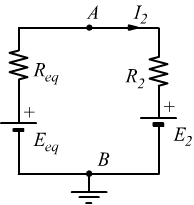
\includegraphics[width=0.3\linewidth]{Immagini/circuito semplificato thevenin.png}
        \caption{circuito semplificato tramite Thevenin}
        \label{fig: circuito semplificato thevenin}
    \end{figure}
    
    A questo punto, la corrente circolante nel circuito semplificato è
    \begin{equation}
        I_2=\frac{E_{eq}-E_2}{R_{eq}+R_2}.
    \end{equation}
\end{ex}

\paragraph{Teorema di Norton.} Un teorema molto simile al teorema \ref{teo: thevenin} è il teorema di Norton, utile anch'esso per la risoluzione di circuiti lineari.
\begin{teo}[teorema di Norton]
    Una rete lineare con due terminali A-B può essere sostituita da un circuito equivalente con un generatore di corrente $I_N$ in parallelo ad un resistore $R_N$.
\end{teo}
\begin{ex}
    Si consideri il seguente circuito.
    \begin{figure}[h]
        \centering
        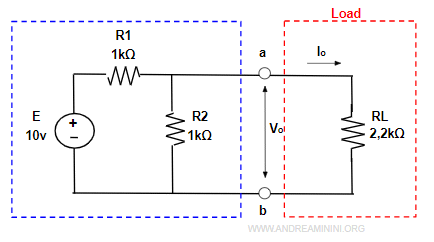
\includegraphics[width=0.55\linewidth]{Immagini/circuito norton.png}
        \caption{circuito risolvibile con il teorema di Norton.}
        \label{fig: circuito norton}
    \end{figure}
    
    Si procede con il cortocircuitare i terminali A-B, in modo da poter calcolare la corrente ai terminali. Tramite la prima legge di Ohm si ha
    \begin{equation}
        I_0=V/R_1=I_N,
    \end{equation}
    che corrisponde alla corrente del generatore equivalente. Per il calcolo del resistore equivalente $R_N$ si mette in cortocircuito il generatore di tensione. Poi si applica una tensione di 1 V in entrata sui morsetti A-B. Quindi, la resistensza di Norton è
    \begin{equation}
        R_N=\frac{R_1R_2}{R_1+R_2}.
    \end{equation}
    A questo punto risolvere il circuito diventa semplice.
\end{ex}

\paragraph{Teorema del massimo trasferimento di potenza.} Il seguente teorema stabilisce la condizione ottimale affinché un generatore trasferisca la massima potenza possibile a un carico collegato.
\begin{teo}[teorema del massimo trasferimento di potenza]
    Per ottenere la massima potenza esterna da un generatore con una resistenza interna finita, la resistenza del carico deve essere uguale alla resistenza del generatore vista dai suoi terminali di uscita.
\end{teo}
Per dimostrare il teorema di parte derivando l'espressione della potenza rispetto alla resistenza di carico e porla uguale a zero, quindi
\begin{equation}
    \frac{dP_c}{dR_c}=\frac{(R_{th}+R_c)^2 -2(R_{th}+R_c)R_c}{(R_{th}+R_c)^4}=0,\quad P_c=\frac{E_{th}^2}{(R_{th}+R_c)^2}R_c.
\end{equation}
Semplificando, si ha 
\begin{equation}
    R_{th}+R_c-2R_c=0\quad\therefore\quad R_c=R_{th}.
\end{equation}
Il teorema comporta il massimo trasferimento di potenza attraverso il circuito e non il massimo rendimento. Se la resistenza del carico è maggiore della resistenza del generatore allora il rendimento è più elevato, poiché viene trasferita al carico una percentuale maggiore della potenza del generatore, ma il valore della potenza sul carico è minore poiché aumenta la resistenza totale del circuito. 
    
Se la resistenza del carico è minore della resistenza del generatore, allora la maggior parte della potenza finisce per essere dissipata nel generatore e, sebbene la potenza totale dissipata sia maggiore, a causa della minore resistenza totale, si scopre che la potenza dissipata nel carico si riduce. Infatti, dato che
\begin{equation}
    \eta=\frac{P_c}{P_{gen}}=\left(\frac{E_{th}}{R_{th}+R_c}\right)^2R_c\frac{R_{th}+R_c}{E_{th}^2}=\frac{R_c}{R_{th}+R_c},
\end{equation}
se $R_{th}=R_c$, allora $\eta=50\%$. La metà della potenza viene dissipata dal circuito equivalente di Thevenin. Per avere $\eta_{max}$ si deve avere $R_c\gg R_{th}$. In sintesi,
\begin{equation}
\eta=
    \begin{cases}
        \dfrac{1}{2}\quad se\quad R_c=R_{th} \\
        0\quad se\quad R_c=0 \\
        1\quad se\quad R_c\to\infty \vee R_{th}=0
    \end{cases}.
\end{equation}

\paragraph{Teorema di Millman.} Il seguente teorema fornisce una formula diretta per determinare la tensione ai capi di un nodo comune a più rami, ognuno costituito da una sorgente di tensione in serie con una resistenza.
\begin{teo}[teorema di Millman]
    La tensione ai capi del bipolo della rete è data dal rapporto tra la somma algebrica delle correnti di corto circuito dei singoli rami e la somma delle conduttanze di ogni ramo. In formule
    \begin{equation}
        V=\frac{\sum_{k}{i_{cc,k}}}{\sum_{k}{G_k}},\quad G_k=R_k^{-1}.
    \end{equation}
\end{teo}
\begin{ex}
    Si consideri il seguente circuito.
\begin{figure}[h]
    \centering
    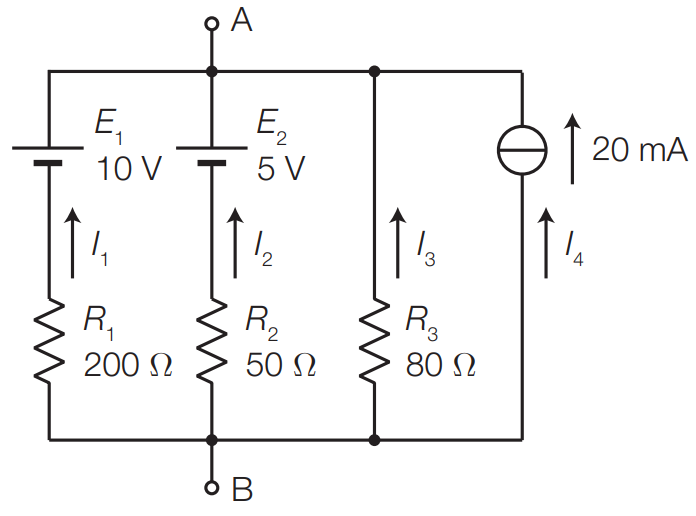
\includegraphics[width=0.5\linewidth]{Immagini/circuito millman.png}
    \caption{circuito risolvibile con il teorema Millman.}
    \label{fig: cirucito millman}
\end{figure}

Le correnti di cortocircuito dei singoli rami sono
    \begin{equation}
        \begin{cases}
            I_{CC,1}=\dfrac{E_1}{R_1}=\SI{50}{mA} \\[2ex]
            I_{CC,2}=-\dfrac{E_2}{R_2}=-\SI{100}{mA} \\[2ex]
            I_{CC,3}=\SI{0}{mA} \\[2ex]
            I_{CC,4}=\SI{20}{mA}
        \end{cases}.
    \end{equation}
    La tensione AB vale quindi
    \begin{equation}
        V_{AB}=\frac{\sum_{i=1}^4{I_{CC,i}}}{\sum_{j=1}^3{R_j^{-1}}}=-\SI{0.8}{V}.
    \end{equation}
    Le correnti nei rami valgono
    \begin{equation}
        \begin{cases}
            I_1=\dfrac{E_1-V_{AB}}{R_1}=\SI{54}{mA} \\[2ex]
            I_2=\dfrac{-E_2-V_{AB}}{R_2}=-\SI{84}{mA} \\[2ex]
            I_3=\dfrac{-V_{AB}}{R_3}=\SI{10}{mA} \\[2ex]
            I_4=\SI{20}{mA}
        \end{cases}.
    \end{equation}
\end{ex}

\section{Tensione alternata}
Un'onda sinusoidale si può rappresentare come una funzione oscillante del tipo
\begin{equation}
    v(t)=V_A\sin{\omega t},\quad\omega=2\pi f=\frac{2\pi}{T}.
\end{equation}
Poiché non è necessario che l'onda passi per l'origine, in generale l'onda può avere un fase $\varphi$ intrinseca, 
\begin{equation}
    \label{eq: onda sinusoidale}
    v(t)=V_A\sin{(\omega t\pm\varphi)}=V_A\sin{\left(\omega t\pm\frac{2\pi\Delta t}{T}\right)}.
\end{equation}
Quando $\varphi<0$ l'onda è in ritardo di fase, invece se $\varphi>0$ è in anticipo di fase. In particolare, se $\varphi=\pm\pi/2$ le onde sono in quadratura di fase, invece se $\varphi=\pm\pi$ sono in opposizione di fase. In generale, la forma d'onda può comprende anche un off-set $V_0$ corrispondente ad un termine additivo, per cui
\begin{equation}
    v(t)=V_A\sin{\left(\omega t\pm\frac{2\pi\Delta t}{T}\right)}+V_0.
\end{equation}
In pratica, $V_0$ corrisponde al punto intorno al quale l'onda oscilla, infatti $\braket{v(t)}=V_0$. 
\begin{obs}
    I generatori di tensione alternata vengono indicati con un cerchio al cui interno viene specificato il tipo di funzione che segue la tensione (sinusoidale, quadra, triangolare...).
\end{obs}
\subsection{Metodo dei fasori}
Considerando un'onda sinusoidale, come quella dell'equazione \eqref{eq: onda sinusoidale}, e usando la formula di addizione del seno si trova
\begin{equation}
    \bm{v}(t)=\bm{v}_A\sin{(\omega t+\varphi)}=\bm{v}_A\left(\cos\varphi \sin{\omega t}+\sin{\varphi}\cos{\omega t}\right)
\end{equation}
Dato che si considera l'ampiezza dell'onda un vettore si può scrivere
\begin{equation}
    \bm{v}_A=\bm{V}_A(\cos{\varphi},\sin{\varphi})=(V_x,V_y).
\end{equation}
In ogni caso, per semplificare i calcoli è possibile sfruttare gli esponenziali per riscrivere i termini oscillanti. Si ricordi l'identità di Eulero
\begin{equation}
    \label{eq: id. eulero}
    e^{j\theta}=\cos\theta+j\sin{\theta}.
\end{equation}
Applicando l'equazione \eqref{eq: id. eulero} all'espressione \eqref{eq: onda sinusoidale} si ottiene
\begin{equation}
    v(t)=V_A\sin{(\omega t+\varphi)}=\Im\left(V_Ae^{j(\omega t+\varphi)}\right)=\Im\left(V_Ae^{j\varphi}e^{j\omega t}\right)
\end{equation}
La quantità $V_Ae^{j\varphi}=V$ è il fasore. Ricordando inoltre che $\Im(A)+\Im(B)=\Im(A+B)$, considerando due tensioni alternate si ottiene
\begin{equation}
    \Im\left(\left[V_Ae^{j\varphi_A}+V_Be^{j\varphi_B}\right]e^{j\omega t}\right),
\end{equation}
dove si nota come siano i fasori a sommarsi. Inoltre, 
\begin{equation}
    V=V_Ae^{j\varphi}=V_A(\cos{\varphi}+j\sin{\varphi})=V_x+jV_y,
\end{equation}
dove $V_A^2=V_x^2+V_y^2$ e $\varphi=\arctan{\left(V_y/V_x\right)}$.
\begin{ex}
    Si consideri il seguente circuito.
    \begin{figure}[h]
        \centering
        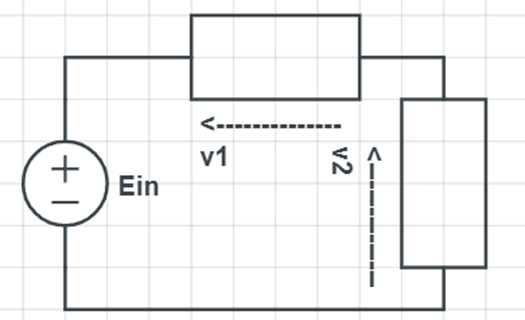
\includegraphics[width=0.45\linewidth]{Immagini/circuito fasori.png}
        \caption{esempio di circuito in tensione alternata.}
        \label{fig: circuito fasori}
    \end{figure}
    
    Le tensioni ai due capi degli elementi
    \begin{equation}
        \begin{cases}
        \label{f circuito semplificato thevenin}
            v_1(t)=V_1\sin{(\omega t+\ang{30})},\quad V_1=\SI{50}{\volt} \\
            v_2(t)=V_2\sin{(\omega t+\ang{60})},\quad V_2=\SI{30}{\volt}
        \end{cases}.
    \end{equation}
    I due fasori corrispondenti sono 
    \begin{equation}
        \begin{cases}
            V'_1=V_1(\cos{\ang{30}}+j\sin{\ang{30}}) \\
            V'_2=V_2(\cos{\ang{60}}+j\sin{\ang{60}})
        \end{cases}.
    \end{equation}
    Quindi, l'ampiezza della tensione in ingresso è
    \begin{equation}
        E_{in}=V_1+V_2=[(43+15)+j(25+26)]=(58+j51)\,\mathrm{V}.
    \end{equation}
    Dunque, la tensione in ingresso è 
    \begin{equation}
        e_{in}(t)=\sqrt{58^2+51^2}\sin{\left(\omega t+\arctan{\frac{51}{58}}\right)}=77\sin{\left(\omega t+\ang{41}\right)}\,\mathrm{V}.
    \end{equation}
\end{ex}

\subsection{Carica e scarica di un condensatore}
\paragraph{Carica.} Il processo di carica di un condensatore non è istantaneo e il tempo di carica dipende dalla resistenza complessiva del generatore e da quella dei conduttori usati per collegare il condensatore al generatore. Nel circuito in figura \ref{fig: car. scar. cond.} quando l'interruttore è aperto non circola corrente e il condensatore non può caricarsi. Al tempo $t=0$ l'interruttore viene chiuso e inizia il processo di carica.
\begin{figure}[ht]
    \centering
    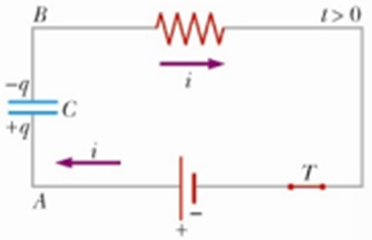
\includegraphics[width=0.35\linewidth]{Immagini/circuito carica-scarica cond-.png}
    \caption{circuito per carica di un condensatore.}
    \label{fig: car. scar. cond.}
\end{figure}

Ad un generico istante di tempo $t$ si ha
\begin{equation}
    \epsilon=v_R+v_C=Ri+\frac{q(t)}{C}=R\frac{dq}{dt}+\frac{q(t)}{C}\quad\therefore\quad \frac{dq}{q-\epsilon C}=-\frac{dt}{RC}.
\end{equation}
Integrando l'equazione tra $t=0$ e un istante $t$ e tra 0 e $q$ si ottiene
\begin{equation}
    \label{eq: q carica cond.}
    \int_{0}^{q}\frac{dq}{q-\epsilon C}=-\frac{1}{RC}\int_{0}^{t}dt\quad\Rightarrow\quad q(t)=\epsilon C(1-e^{-t/\tau}),
\end{equation}
dove $\tau=RC$ è il tempo caratteristico.  Derivando l'equazione di $q(t)$ rispetto al tempo si può ricavare la corrente $i(t)$ come
\begin{equation}
    \label{eq: corrente carica cond.}
    i(t)=\frac{dq}{dt}=\frac{\epsilon}{R}e^{-t/\tau}.
\end{equation}
Moltiplicando per $R$ l'equazione \eqref{eq: corrente carica cond.} si ricava la tensione ai capi del resistore
\begin{equation}
    v_R=Ri=\epsilon e^{-t/\tau}.
\end{equation}
Dividendo per $C$ l'equazione \eqref{eq: q carica cond.} si ricava la tensione ai capi del condensatore
\begin{equation}
    \label{eq: tensione cond. carica}
    v_C=\frac{q(t)}{C}=\epsilon\left(1-e^{-t/\tau}\right).
\end{equation}
Inoltre, dalle equazioni \eqref{eq: corrente carica cond.} e \eqref{eq: tensione cond. carica} si può disegnare il grafico delle due funzioni per $t\to\infty$. Quindi, moltiplicando per $i$ la relazione $\epsilon=v_R+v_C$ si ottiene una relazione tra potenze
\begin{equation}
    P_{gen}=P_R+P_C.
\end{equation}
La potenza assorbita dal generatore è in parte dissipata sulla resistenza e in parte assorbita dal condensatore, in linea con il principio di conservazione dell'energia.
\begin{equation}
    \begin{cases}
        P_{gen}=\epsilon i=\dfrac{\epsilon^2}{R}e^{-t/\tau} \\[2ex]
        P_R=Ri^2=\dfrac{\epsilon^2}{R}e^{-2t/\tau} \\[2ex]
        P_C=P_{gen}-P_R=\dfrac{\epsilon^2}{R}e^{-t/\tau}\left(1-e^{-t/\tau}\right)
    \end{cases}
\end{equation}
Alla fine della carica, il lavoro erogato dal generatore, l'energia dissipata dalla resistenza e quella immagazzinata nel condensatore valgono
\begin{equation}
    \begin{cases}
        W_{gen}=\dfrac{\epsilon^2}{R}\int_{0}^{\infty}e^{-t/\tau}dt=C\epsilon^2 \\[2ex]
        U_R=\dfrac{\epsilon^2}{R}\int_{0}^{\infty}e^{-2t/\tau}dt=\dfrac{1}{2}C\epsilon^2 \\[2ex]
        U_C=W_{gen}-U_R=\dfrac{1}{2}C\epsilon^2.
    \end{cases}
\end{equation}
Nel processo di carica metà dell'energia spesa dal generatore viene dissipata in calore e metà immagazzinata nel condensatore.

\paragraph{Scarica.} Se all'istante $t=0$, nel circuito in figura \ref{fig: scar. cond.}, l'interruttore viene chiuso inizia il processo di scarica attraverso la resistenza $R$.
\begin{figure}[h]
    \centering
    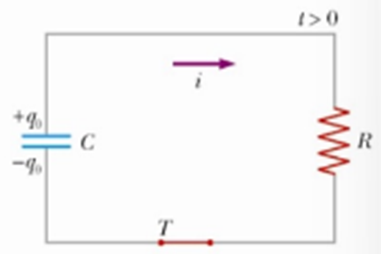
\includegraphics[width=0.35\linewidth]{Immagini/circuito scarica cond.png}
    \caption{circuito per scarica condensatore.}
    \label{fig: scar. cond.}
\end{figure}

La tensione ai capi del condensatore è
\begin{equation}
    v_C=v_R\quad\Rightarrow\quad\frac{q}{C}=Ri=-R\frac{dq}{dt}.
\end{equation}
Si noti come la corrente ha segno negativo in quanto la carica diminuisce nel tempo e $Ri>0$ se la corrente è positiva. Quindi
\begin{equation}
    \label{eq: q scarica cond.}
    \int_{q_0}^{q}\frac{dq}{q}=-\int_{0}^{r}\frac{dt}{\tau}\quad\Rightarrow\quad q(t)=q_0e^{-t/\tau}.
\end{equation}
Moltiplicando l'equazione \eqref{eq: q scarica cond.} per $C$ si ottiene la differenza di potenziale ai capi del condensatore
\begin{equation}
    \label{eq: tens. scar. cond.}
    v_C=\frac{q(t)}{C}=V_0e^{-t/\tau}.
\end{equation}
La corrente vale
\begin{equation}
    \label{eq: corrente scar. cond.}
    i(t)=\frac{dq}{dt}=\frac{V_0}{R}e^{-t/\tau}.
\end{equation}
La potenza dissipata su $R$ vale
\begin{equation}
    P_R=Ri^2=\frac{V_0^2}{R}e^{-2t/\tau}.
\end{equation}
L'energia dissipata nel processo di scarica del condensatore vale
\begin{equation}
    W_R=\frac{V_0^2}{R}\int_{0}^{\infty}e^{-2t/\tau}dt=\frac{1}{2}CV_0^2.
\end{equation}
Inoltre, dalle equazioni \eqref{eq: corrente scar. cond.} e \eqref{eq: tens. scar. cond.} si può disegnare il grafico delle due funzioni per $t\to\infty$. 

\subsection{Tensione ai capi degli elementi circuitali}
\paragraph{Tensione ai capi di un condensatore.} Si consideri il circuito in figura \ref{fig: alt. cond.}. Per costruzione 
\begin{equation}
    v_{in}=v_R+v_{out}=IR+v_C.
\end{equation}
\begin{figure}[h]
    \centering
    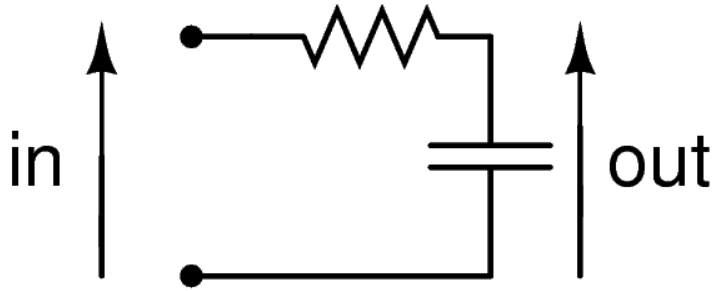
\includegraphics[width=0.3\linewidth]{Immagini/alt. cond..png}
    \caption{circuito in alternata con condensatore.}
    \label{fig: alt. cond.}
\end{figure}

Poiché $v_C=q/C$, riarragiando e derivando si ottiene
\begin{equation}
    \frac{dq}{dt}=C\frac{dv_C}{dt}=i.
\end{equation}
Approssimando ora $v_{out}\ll v_{in}$ segue che
\begin{equation}
    v_{in}=RC\frac{dv_{out}}{dt}.
\end{equation}
Risolvendo per $v_{out}$ si ottiene
\begin{equation}
    v_{out}=\frac{1}{RC}\int v_{in}dt=\frac{1}{\tau}\int v_{in}dt.
\end{equation}
Più $\tau$ è grande, più l'andamento della tensione approssima una retta. Se $\tau$ invece non è così grande da permettere l'approssimazione, l'andamento della tensione sarà meglio approssimata dall'esponenziale.

\paragraph{Tensione ai capi di un resistore.} Si consideri il circuito in figura \ref{fig: alt. res.}. Per costruzione
\begin{equation}
    v_{in}=v_{out}+v_C.
\end{equation}
\begin{figure}[h]
    \centering
    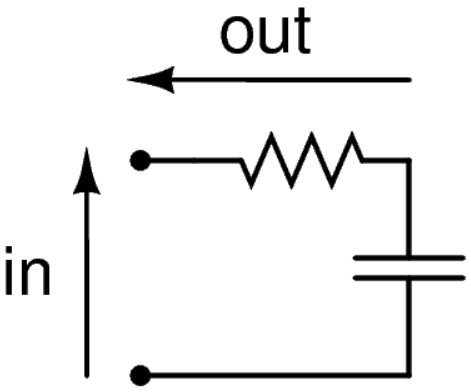
\includegraphics[width=0.22\linewidth]{Immagini/alt. res..png}
    \caption{Circuito in alternata con resistenza.}
    \label{fig: alt. res.}
\end{figure}

Poiché 
\begin{equation}
    v_C=\frac{q}{C}=\frac{1}{C}\int idt=\frac{1}{RC}\int Rv_Cdt=\frac{1}{\tau}\int v_Rdt.
\end{equation}
Approssimando $v_{out}\ll v_{in}$ segue che
\begin{equation}
    v_{in}=\frac{1}{\tau}\int v_{out}dt\quad\Rightarrow\quad v_{out}=\tau\frac{dv_{in}}{dt}.
\end{equation}

\paragraph{Tensione ai capi di un induttore.} Un induttore è un dispositivo utilizzato per generare un campo magnetico, al passaggio di corrente elettrica, in una regione dello spazio. La tensione ai capi dell'induttore vale
\begin{equation}
    v_L(t)=L\frac{di}{dt},
\end{equation}
dove $L$ è l'induttanza, la cui unità di misura è l'Henry [H]. Si consideri il circuito in figura \ref{fig: alt. ind.}.
\begin{figure}[h]
    \centering
    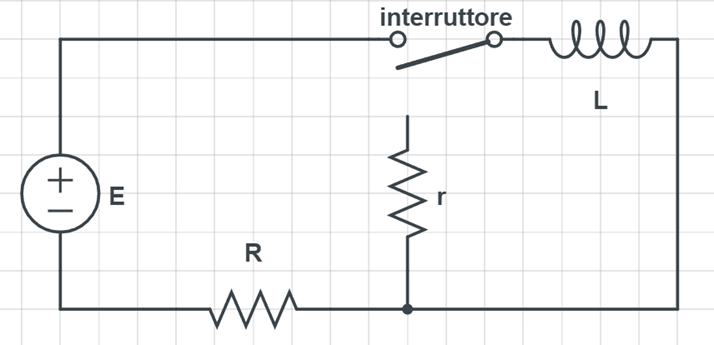
\includegraphics[width=0.5\linewidth]{Immagini/alt. ind..png}
    \caption{circuito in alternata con induttore.}
    \label{fig: alt. ind.}
\end{figure}

Quando il circuito è chiuso l'equazione del circuito è
\begin{equation}
    E=v_L+v_R=L\frac{di}{dt}+Ri.
\end{equation}
Risolvendo l'equazione differenziale, si ha
\begin{equation}
    L\int_{0}^{i}\frac{di}{Ri-E}=-\int_{0}^{t}dt\quad\Rightarrow\quad\frac{L}{R}\ln{\frac{Ri-E}{-E}}=-t.
\end{equation}
Si può verificare che il rapporto tra induttanza e resistenza è dimensionalmente un tempo; dunque, è possibile identificare questa quantità come il tempo caratteristico dei circuiti RL
\begin{equation}
    \tau=\frac{L}{R}.
\end{equation}
Dunque, la corrente attraverso l'induttanza quando il circuito è chiuso è
\begin{equation}
    i(t)=\frac{E}{R}\left(1-e^{-t/\tau}\right).
\end{equation}
La corrente $i$ dunque segue l'andamento di un esponenziale crescente con un asintoto per $t\to\infty$ a $E/R$. Inoltre, la tensione ai suoi capi è
\begin{equation}
    v_L=Ee^{-t/\tau}.
\end{equation}
Quando il circuito è aperto invece l'equazione del circuito è
\begin{equation}
    v_r+v_L=ri+L\frac{di}{dt}=0.
\end{equation}
Al tempo $t=0$ si ha $i(t_0)=i_0$ che è la corrente alla fine del processo di carica; invece, al generico tempo $t$ si ha una generica corrente $i(t)$. Risolvendo l'equazione si ha che la corrente quando il circuito è aperto è 
\begin{equation}
    i(t)=i_0e^{-t/\tau'},
\end{equation}
dove $\tau'=L/r$. La tensione ai capi dell'induttore ora è invece data da
\begin{equation}
    v_L(t)=-i_0re^{-t/\tau'}=\frac{-rE}{R}e^{-t/\tau'}.
\end{equation}
La corrente quando il circuito è chiuso ha verso nel senso orario. Stessa cosa quando il circuito è aperto. A differenza del caso del condensatore, la corrente non cambia verso di percorrenza passando dal processo di carica a quello di scarica. A cambiare segno ora è invece la tensione, come si nota dal segno meno nell'ultima equazione. Quindi nell'induttanza la corrente è continua e la tensione è discontinua, nel conduttore la tensione è continua e la corrente è discontinua.

È possibile considerare $r\gg R$, in questo modo la tensione ai capi dell'induttanza sarà molto alta. Con $r\to\infty$, ovvero nella pratica si considera il circuito aperto, la tensione è così grande che viene superata la rigidità del dielettrico, in questo caso l'aria.

\subsection{Condensatori e induttori in serie e in parallelo}
\paragraph{Condensatori in parallelo.} Si consideri il seguente circuito.
\begin{figure}[H]
    \centering
    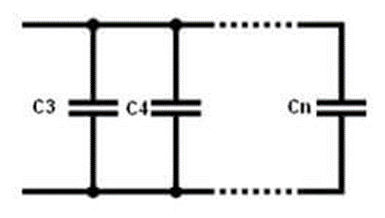
\includegraphics[width=0.3\linewidth]{Immagini/cond. parallelo.png}
    \caption{condensatori in parallelo.}
    \label{fig: cond. parallelo}
\end{figure}

Dividendo la corrente in ulteriori $n$ correnti e usando l'equazione \eqref{eq: sumI=0},
\begin{equation}
    i(t)=i_1+\cdots+i_n,
\end{equation}
si ha per il singolo condensatore
\begin{equation}
    v=\frac{q_j}{C_j}\quad\Rightarrow\quad i_j(t)=C_j\frac{dv}{dt}.
\end{equation}
Quindi
\begin{equation}
    i(t)=C_1\frac{dv}{dt}+\cdots+C_n\frac{dv}{dt}=\sum_{j=1}^n C_j\frac{dv}{dt}.
\end{equation}
Dunque
\begin{equation}
    C_{eq}=\sum_{j=1}^n C_j.
\end{equation}

\paragraph{Condensatori in serie.} Si consideri il seguente circuito.
\begin{figure}[h]
    \centering
    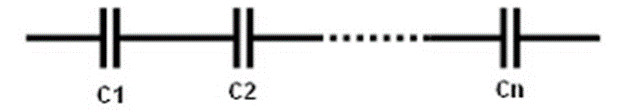
\includegraphics[width=0.5\linewidth]{Immagini/cond. serie.png}
    \caption{condensatori in serie.}
    \label{fig: cond. serie}
\end{figure}

Per costruzione
\begin{equation}
    v(t)=v_1+\cdots+v_n.
\end{equation}
Per il singolo condensatore si ha
\begin{equation}
    v_j=\frac{1}{c_j}\int i_jdt.
\end{equation}
Quindi
\begin{equation}
    v(t)=\frac{1}{C_1}\int idt+\cdots+\frac{1}{C_n}\int idt=\sum_{j=1}^n\frac{1}{C_j}\int idt.
\end{equation}
Dunque
\begin{equation}
    C_{eq}=\left(\sum_{j=1}^n\frac{1}{C_j}\right)^{-1}.
\end{equation}

\paragraph{Induttori in serie.} Si consideri il seguente circuito.
\begin{figure}[h]
    \centering
    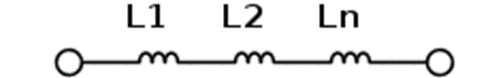
\includegraphics[width=0.4\linewidth]{Immagini/ind. serie.png}
    \caption{induttori in serie.}
    \label{fig: ind. serie}
\end{figure}

Per costruzione
\begin{equation}
    v(t)=v_1+\cdots+v_n.
\end{equation}
Per il singolo induttore si ha
\begin{equation}
    v_j=L_j\frac{di}{dt}.
\end{equation}
Quindi
\begin{equation}
    v(t)=L_1\frac{di}{dt}+\cdots+L_n\frac{di}{dt}=\sum_{j=1}^n L_j\frac{di}{dt}.
\end{equation}
Dunque
\begin{equation}
    L_{eq}=\sum_{j=1}^n L_j.
\end{equation}

\paragraph{Induttori in parallelo.} Si consideri il seguente circuito.
\begin{figure}[h]
    \centering
    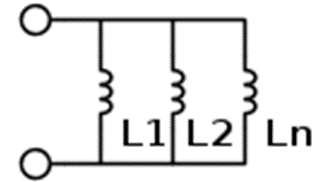
\includegraphics[width=0.25\linewidth]{Immagini/ind. parallelo.png}
    \caption{induttori in parallelo.}
    \label{fig: ind. parallelo}
\end{figure}

Per costruzione 
\begin{equation}
    i(t)=i_1+\cdots+i_n.
\end{equation}
Per il singolo induttore si ha
\begin{equation}
    i_j=\frac{1}{L_j}\int vdt.
\end{equation}
Quindi
\begin{equation}
    i(t)=\frac{1}{L_1}\int vdt+\cdots+\frac{1}{L_n}\int vdt=i(t)=\sum_{j=1}^n\frac{1}{L_j}\int vdt.
\end{equation}
Dunque
\begin{equation}
    L_{eq}=\left(\sum_{j=1}^n\frac{1}{L_j}\right)^{-1}.
\end{equation}

\subsection{Risposta degli elementi circuitali}
\paragraph{Risposta dei resistori.} Si consideri una resistenza isolata. La tensione ai capi di essa vale
\begin{equation}
    v_R(t)=i_RR=I_RR\sin{\omega t}=|V_R|\sin{\omega t}=\Im\left(V_Re^{j\omega t}\right).
\end{equation}
Il fatto di avere la resistenza non induce sfasamento tra la corrente e la tensione, $\varphi=0$. Per un elemento puramente resistivo, il voltaggio ai capi e la corrente attraverso l'elemento sono in fase, con i loro massimi collegati dalla legge di Ohm.

\paragraph{Risposta degli induttori.} Si consideri un induttore isolata. La tensione ai capi di esso vale
\begin{equation}
    v_L(t)=L\frac{di_L}{dt}=I_L\omega L\cos{\omega t}=|V_L|\sin{\left(\omega t+\frac{\pi}{2}\right)}.
\end{equation}
Questo significa che la corrente e la tensione non sono in fase, viene infatti indotto uno sfasamento, in particolare la corrente è in anticipo di $\pi/2$.
\begin{equation}
    v_L(t)=\Im(I_L\omega Le^{j\left(\omega t+\pi/2\right)})=\Im(jI_L\omega Le^{j\omega t})=V_Le^{j\omega t}.
\end{equation}
La reattanza dell'induttore è definita come
\begin{equation}
    X_L=\omega L.
\end{equation}
Mentre, l'impedenza è definita come
\begin{equation}
    Z_L=jX_L=j\omega L.
\end{equation}

\paragraph{Risposta dei condensatori.} Si consideri un condensatore isolato. La tensione ai capi del condensatore vale
\begin{equation}
    v_C(t)=\frac{q(t)}{C}=q(t)\int i_Cdt=\frac{-I_C}{\omega C}\cos{\omega t}=|V_C|\sin{\left(\omega t-\frac{\pi}{2}\right)}.
\end{equation}
In questo caso viene indotto uno sfasamento tra tensione e corrente, in particolare la tensione è in ritardo rispetto alla corrente di $-\pi/2$.
\begin{equation}
    v_C(t)=\Im\left(\frac{I_C}{\omega C}e^{j\left(\omega t-\pi/2\right)}\right)=\Im\left(\frac{-jI_C}{\omega C}e^{j\omega t}\right)=\Im\left(V_Ce^{j\omega t}\right).
\end{equation}
La reattanza del condensatore è definita come
\begin{equation}
    X_C=(-)\frac{1}{\omega C},
\end{equation}
dove il segno meno è una convenzione non sempre rispettata. L'impedenza del condensatore è definita come
\begin{equation}
    Z_C=jX_C=\frac{-j}{\omega C}.
\end{equation}

\subsection{Impedenza e risonanza}
L'impedenza $Z$, in elettrotecnica, è una grandezza fisica che rappresenta l'opposizione di un circuito al passaggio di una corrente elettrica alternata, esprimibile come numero complesso. Infatti, ponendo in serie una resistenza, un induttore e un condensatore si ottiene che la caduta di potenziale vale
\begin{equation}
    V=\left(R+j\omega L-\frac{j}{\omega C}\right)I=ZI,
\end{equation}
dove $Z=R+jX$ è appunto l'impedenza. 

La tensione chiaramente è sfasata rispetto alla corrente, tale sfasamento è dato da
\begin{equation}
    \varphi=\arctan{\frac{X}{R}}=\arctan{\left(\frac{\omega L-\frac{1}{\omega C}}{R}\right)}.
\end{equation}
In termini della pulsazione della $fem$ applicata la corrente ha un massimo in corrispondenza della pulsazione propria della serie RLC. Infatti, la corrente
\begin{equation}
    i_0=\frac{\epsilon}{\sqrt{R^2+\left(\omega L-\frac{1}{\omega C}\right)^2}},
\end{equation}
quando
\begin{equation}
    \omega L-\frac{1}{\omega C}=0\quad\Rightarrow\quad\omega=\omega_0=\frac{1}{\sqrt{LC}},
\end{equation}
assume il valore massimo
\begin{equation}
    i_{0,max}=\frac{\epsilon}{R}
\end{equation}
e lo sfasamento è nullo 
\begin{equation}
    \tan{\varphi}=\frac{\omega_0-\frac{1}{\omega_0C}}{R}=0.
\end{equation}
Dunque, il circuito si comporta come se il carico fosse puramente resistivo.
\begin{defn}[larghezza di risonanza]
    Si definisce larghezza di risonanza la differenza tra i valori $\omega_2$ e $\omega_1$ in corrispondenza dei quali la corrente massima vale $\epsilon/R\sqrt{2}$. 
\end{defn}
I due valori 
    \begin{equation}
        \omega_2=\frac{R}{2L}+\sqrt{\frac{R^2}{4L^2}+\omega_0^2},\quad\omega_1=\frac{-R}{2L}+\sqrt{\frac{R^2}{4L^2}+\omega_0^2},
    \end{equation}
non sono equidistanti da $\omega_0$ e dunque, la curva non è simmetrica. La larghezza della curva di risonanza vale
\begin{equation}
    \Delta\omega=\omega_2-\omega_1=\frac{R}{L}.
\end{equation}
\begin{defn}[fattore di merito]
    Il fattore di merito $Q$ della risonanza è dato da
    \begin{equation}
        Q=\frac{\omega_0}{\Delta\omega}=\frac{\omega_0L}{R}.
    \end{equation}
\end{defn}
Il fattore $Q$ è tanto maggiore quanto più stretta è la risonanza. Un circuito RLC con un alto valore di $Q$ è molto selettivo, ovvero la corrente circola solo se la pulsazione della $fem$ in ingresso è molto vicina a quella propria.

\subsection{Potenza variabile}
Si consideri una corrente entrante in un dispositivo
\begin{equation}
    \begin{cases}
        i(t)=I\sin{(\omega t)} \\
        v(t)=V\sin{(\omega t+\varphi)}
    \end{cases}.
\end{equation}
La potenza istantanea $p(t)$ vale
\begin{equation}
\begin{split}
    p(t)&=VI\sin{(\omega t)}\sin{(\omega t+\varphi)}=VI\sin{\omega t}(\sin{\omega t}\cos{\varphi}+\sin{\varphi}\cos{\omega t})\\
        &=VI\sin^2{(\omega t)}\cos{\varphi}+VI\sin{(\omega t)}\cos{(\omega t)}\sin{\varphi} \\
        &=\underbrace{\frac{VI}{2}\cos{(\varphi)}}_{\substack{potenza \\ reale}}(1-\cos{2\omega t})+\underbrace{\frac{VI}{2}\sin{(\varphi)}}_{\substack{potenza \\ reattiva}}\sin{(2\omega t)}.
\end{split}
\end{equation}
La potenza media $\langle p(t)\rangle$ coincide con la potenza reale e quindi vale
\begin{equation}
    \langle p(t)\rangle=P=\frac{VI}{2}\cos{\varphi}.
\end{equation}
Questo perché il valor medio di $\sin{(2\omega t)}$ è zero, mentre quello di $\cos{(2\omega t)}$ è 1. Dalle definizioni, rispettivamente di tensione e corrente efficace
\begin{equation}
    V_{eff}=\dfrac{V}{\sqrt{2}},\quad I_{eff}=\dfrac{I}{\sqrt{2}},
\end{equation}
si ricava la formula di Galileo Ferraris 
\begin{equation}
    \label{eq: galileo ferraris}
    P=V_{eff}I_{eff}\cos{\varphi},
\end{equation}
dove il termine $\cos{\varphi}$ è detto fattore di potenza. Sostituendo in \eqref{eq: galileo ferraris} i termini
\begin{equation}
    \cos{\varphi}=\dfrac{R}{Z},\quad V_{eff}=ZI_{eff},
\end{equation}
si ottengono altre due forme dell'equazione \eqref{eq: galileo ferraris}
\begin{equation}
    \label{eq: galileo ferraris 2}
        P=RI_{eff}^2=\dfrac{V_{eff}^2}{Z}\cos{\varphi},\quad Z=\sqrt{R_{TOT}^2+X_{TOT}^2}.
\end{equation}
Dall'equazione \eqref{eq: galileo ferraris 2} si deduce che la potenza media viene dissipata solo dagli elementi resistivi. L'ampiezza della potenza reattiva vale
\begin{equation}
    Q=\frac{VI}{2}\sin{\varphi}=V_{eff}I_{eff}\sin{\varphi}.
\end{equation}
La potenza apparente è definita come
\begin{equation}
    S=P+jQ,
\end{equation}
il cui modulo vale $|S|=\sqrt{P^2+Q^2}=V_{eff}I_{eff}$. La potenza reale, la potenza apparente e l'ampiezza della potenza reattiva formano un ``triangolo delle potenze'' appartenente al piano complesso. Inoltre, la potenza apparente $S$ è espressa in volt-ampere [VA] e l'ampiezza della potenza reattiva $Q$ è espressa in volt-ampere-reattivi [VAR]. Infine, dalle relazioni di $P$, $Q$ e $S$ si ricava che
\begin{equation}
    \tan{\varphi}=\frac{Q}{P}.
\end{equation}
In sintesi: 
\begin{enumerate}
    \item la potenza attiva è la potenza effettivamente convertita in lavoro utile, ovvero la potenza media effettiva consumata dal carico;
    \item la potenza reattiva è la potenza associata ai campi elettrici e magnetici nei componenti reattivi, come induttori e condensatori. Questa non fa lavoro utile ma oscilla tra il generatore e il carico e può causare perdite nei sistemi elettrici;
    \item la potenza apparente è la somma vettoriale della potenza attiva e reattiva. È la potenza che il generatore deve fornire al circuito, indipendentemente dal fatto che venga usata per lavoro utile o sia immagazzinata temporaneamente negli elementi reattivi. Tiene conto di tutte le forme di energia trasferite, sia quella utile sia quella oscillante.
\end{enumerate}
\begin{figure}[h]
    \centering
    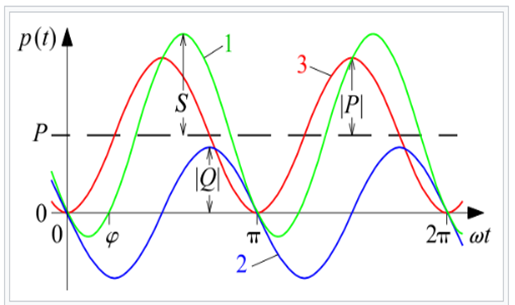
\includegraphics[width=0.55\linewidth]{Immagini/grafici potenze.png}
    \caption{grafico delle potenze.}
    \label{fig: grafico potenze}
\end{figure}
Un circuito RLC per efficiente deve avere $\varphi=0$. In questo modo la potenza reattiva si annulla, massimizzando il valore della potenza reale e minimizzando le perdite di energia. La condizione $\varphi=0$ avviene quando il circuito è in risonanza. 

\subsection{Trasformatore}
Il trasformatore è una macchina elettrica statica, funzionante in corrente alternata e basata sul fenomeno dell'induzione elettromagnetica. Durante la trasformazione c'è sempre una quantità di perdita, che ne determina l'efficienza. \'E una macchina reversibile. Il materiale di cui se ne vede la sezione in figura \ref{fig: schema trasf.} è ferromagnetico, il suo compito è quello di indirizzare il campo magnetico lungo un percorso ben preciso. La differenza di potenziale ai capi delle spire del primario, ovvero dell'induttanza, vale
\begin{equation}
    e_p=N_p\frac{d\Phi_p}{dt}=L_p\frac{i_p}{dt}=N_sA_p\frac{dB_s}{dt}.
\end{equation}
\begin{figure}[h]
    \centering
    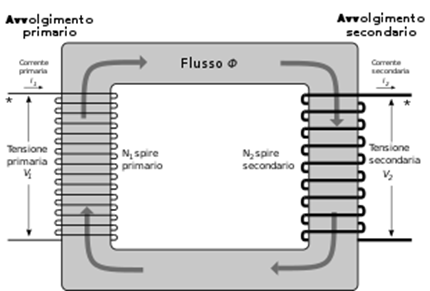
\includegraphics[width=0.5\linewidth]{Immagini/schema trasf..png}
    \caption{schema dei componenti di un trasformatore.}
    \label{fig: schema trasf.}
\end{figure}
\begin{figure}[h]
    \centering
    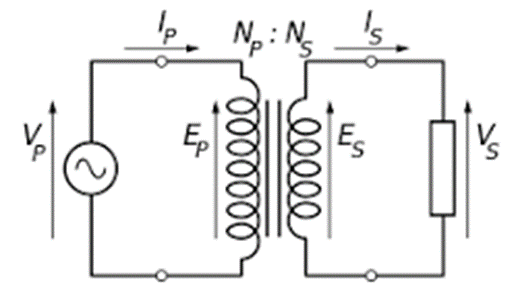
\includegraphics[width=0.5\linewidth]{Immagini/diagramma trasf..png}
    \caption{diagramma circuitale di un trasformatore.}
    \label{fig: diagramma trasf.}
\end{figure}

I due flussi di campo magnetico nel primario e nel secondario sono messi in relazione da un fattore $K$ che vale
\begin{equation}
    K=\frac{\Phi_s}{\Phi_p}\le1.
\end{equation}
Supponendo che $K\approx 1$ per costruzione del sistema, e che le spire abbiano tutte la stessa sezione, allora si ha
\begin{equation}
    \frac{e_p}{e_s}=\frac{N_p}{N_s}.
\end{equation}
Per cui la fase non cambia l'una rispetto all'altra, ovvero sono in fase tra di loro. Se il circuito secondario viene chiuso allora circolerà corrente. Se circola corrente, di conseguenza, si genererà un campo magnetico nelle spire del secondario che indurrà un flusso di campo magnetico opposto a quello del primario. Il generatore di tensione dovrà dunque sopperire a questo effetto. La forza elettromotrice indotta vale
\begin{equation}
    I_{s,p}=M\frac{di_s}{dt}.
\end{equation}
Il coefficiente di mutua induzione $M$ vale 
\begin{equation}
    M=K\sqrt{L_pL_s}.
\end{equation}
La potenza del primario deve essere uguale alla potenza del secondario, ossia $P_p=P_s$. Esprimendo le potenze in funzione della tensione si ottiene
\begin{equation}
    e_pI_p=e_sI_s\quad\Rightarrow\quad\frac{I_p}{I_s}=\frac{N_s}{N_p}.
\end{equation}
\begin{obs}
    Il trasporto di corrente viene effettuato ad alta tensione perché più questa è alta, meno potenza viene dissipata dall'effetto Joule.
\end{obs}

\section{Semiconduttori}
In generale, la resistività dei conduttori e degli isolanti valgono rispettivamente $\rho\approx\SI{e-8}{\Omega m}$ e $\rho\approx\SI{e-13}{\Omega m}$. Tra queste due categorie di materiali si trovano i semiconduttori che possiedono resistività intermedia. I due semiconduttori più comuni e utilizzati sono il silicio e il germanio, di resistività rispettivamente $\rho_{\mathrm{Si}}\approx\SI{e3}{\Omega m}$ e $\rho_\mathrm{Ge}\approx\SI{e-1}{\Omega m}$.

I semiconduttori sono definiti come solidi nei quali a $\SI{0}{K}$ la banda a energia più elevata di stati elettronici occupati è completamente libera. Dato che la conduzione elettrica nei solidi avviene solo quando si ha una banda di stati elettronici non saturata, la conduzione nei semiconduttori puri avviene solo quando gli elettroni sono stati eccitati e portati nelle bande a energia superiore. A temperatura ambiente una porzione molto piccola di elettroni in un semiconduttore è termicamente eccitata e portata dalla banda di valenza, ovvero la banda completa a $\SI{0}{K}$, alla banda di conduzione, la più vicina banda superiore.  L'intervallo che separa queste due bande è detto intervallo proibito e determina la facilità con cui gli elettroni possono essere portati dalla banda di valenza alla banda di conduzione; la grandezza di questo intervallo serve come parametro per distinguere i semiconduttori dagli isolanti. In generale, i semiconduttori hanno un gap di energia di circa $\SI{1}{eV}$ mentre gli isolanti di molte volte maggiori. La temperatura gioca quindi un ruolo importante, infatti all'aumentare di essa corrisponde un incremento dell'agitazione termica degli atomi, e quindi degli elettroni di valenza, che sono dunque facilitati ad attraversare il gap energetico.
\begin{figure}[h]
    \centering
    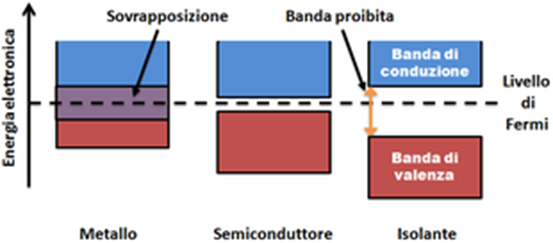
\includegraphics[width=0.6\linewidth]{Immagini/bande elettroniche.png}
    \caption{bande elettroniche.}
    \label{fig: bande elettroniche}
\end{figure}
\begin{obs}
    A temperatura ambiente, ovvero a $\SI{300}{K}$, per il silicio il gap di energia è di $\SI{1.1}{eV}$ e per il germanio è $\SI{0.7}{eV}$.
\end{obs}
Quando in un semiconduttore gli elettroni sono portati dalla banda di valenza alla banda di conduzione, entrambe le bande contribuiscono alla conduzione, al quale può avvenire in ogni banda non completamente piena. Gli elettroni nella banda di conduzione sono chiamati elettroni liberi. Gli stati energetici liberi nella banda di valenza sono chiamati lacune. Benché non siano in effetti delle vere entità fisiche, si può mostrare che hanno un comportamento molto simile a quello di particelle cariche positivamente, e sono usualmente trattate come tali. Gli elettroni possono accedere a livelli vuoti ricevendo energia da un campo elettrico esterno; questo comporta una densità di corrente concorde al campo. Gli elettroni delle bande inferiori, che sono tutte piene (l'ultima è quella di valenza), non acquistano energia e non influiscono nel processo di conduzione. Questa configurazione non è l'unica che permetta di avere proprietà di conduzione. Può accadere che l'ultima banda piena si sovrapponga a quella successiva vuota. Questo tipo di struttura a bande si trova ad esempio nel magnesio e spiega perché questo ha una buona conducibilità elettrica.

Non sono conduttori i solidi refrattari in cui l'ultima banda contenente elettroni è completamente piena e non è sovrapposta alla banda successiva. Questa è la configurazione che caratterizza gli isolanti e i semiconduttori. Attraverso il parametro del gap energetico è quindi possibile definire i semiconduttori come quei solidi la cui banda proibita è abbastanza piccola da far sì che ad una temperatura inferiore al punto di fusione si possa osservare statisticamente una conduzione non trascurabile dovuta al passaggio dei portatori di carica dalla banda di valenza a quella di conduzione per eccitazione termica.

\subsection{Corrente nei semiconduttori}
Gli elettroni passati alla banda di conduzione sotto l'azione di un campo elettrico esterno danno luogo a una densità di corrente $\bm{J}$. Ogni elettrone che passa dalla banda di valenza a quella di conduzione lascia un livello vuoto detto lacuna. In presenza di tale campo, in un semiconduttore si ha un flusso di carica negativa dovuto agli elettroni nella banda di conduzione e uno di carica positiva dovuto alle lacune nella banda di valenza. Ponendo rispettivamente $n_e$, $n_l$ la concentrazione degli elettroni e delle lacune; $\bm{v}_e$ e $\bm{v}_l$ le rispettive velocità di deriva, la prima opposta e la seconda concorde al campo elettrico esterno, si può scrivere la densità di corrente come
\begin{equation}
    \label{eq: j drude}
    \bm{J}=e(n_e\bm{v}_e+n_l\bm{v}_l).
\end{equation}
Secondo il modello di Drude la velocità di deriva in generale è
\begin{equation}
    \label{eq: vel. deriv.}
    \langle\bm{v}_d\rangle=\frac{q\tau}{m}\bm{E}=\mu\bm{E},
\end{equation}
dove $\mu$ è detta mobilità, la cui unità di misura è [cm$^2$V$^{-1}$s$^{-1}$]. Sostituendo l'equazione \eqref{eq: vel. deriv.} nell'equazione \eqref{eq: j drude} si ottiene
\begin{equation}
    \bm{J}=(n_e\mu_e+n_l\mu_l)e\bm{E}=\sigma\bm{E},
\end{equation}
dove $\sigma$ è la conduttività, reciproco della resistività $\rho$.
\begin{defn}[semiconduttore intrinseco]
    Un semiconduttore intrinseco è un semiconduttore sufficientemente puro per cui le impurità non influiscono apprezzabilmente sul suo comportamento elettrico.
\end{defn}
\begin{defn}[semiconduttore estrinseco]
    Un semiconduttore estrinseco è un semiconduttore drogato con impurità per modificare il numero e il tipo dei portatori liberi di carica.
\end{defn}
Per un cristallo intrinseco si ha che $n_e=n_l=n$ e 
\begin{equation}
    n_i=Ck_BT^{3/2}e^{-E_g/2k_BT},
\end{equation}
dove $C$ è una costante che dipende dal materiale. Per i materiali solidi questa relazione è sempre verificata e in generale vale quando $E_g\gg k_BT$.
\begin{obs}
    Per il silicio la mobilità vale $\mu_{\mathrm{Si}}^l=\SI{480}{\cm^2\V^{-1}\s^{-1}}$ e $\mu_{\mathrm{Si}}^e=\SI{1350}{\cm^2\V^{-1}\s^{-1}}$, quindi se $n_e=n_l$ a $\bm{J}$ contribuisce di più il termine di conduzione. Inoltre, a temperatura ambiente $n_{\mathrm{Si}}^i=\SI{1.5e10}{\cm^{-3}}$.
\end{obs}

\subsection{Drogaggio}
Attraverso la procedura di drogaggio si possono ottenere effetti importanti sulle proprietà del reticolo cristallino.
Esistono due tipi di drogaggio: tipo N e tipo P.

\paragraph{Tipo N.} Lo scopo del drogaggio di tipo N è produrre un eccesso di elettroni liberi nel materiale. Nel caso del Si, gli atomi hanno quattro elettroni di valenza, ciascuno dei quali è legato in modo covalente a uno dei quattro atomi adiacenti di Si. Se un atomo con cinque elettroni di valenza, come uno del gruppo 5 della tavola periodica, come il fosforo, è incorporato nel reticolo cristallino al posto di un atomo di Si, allora quell'atomo avrà quattro legami covalenti e un elettrone libero. Questo elettrone aggiuntivo è solo debolmente legato all'atomo e può essere facilmente portato nella banda di conduzione. Già alle normali temperature praticamente tutti questi elettroni sono in banda di conduzione. Poiché l'eccitazione di questi elettroni non crea lacune in banda di valenza, il numero di elettroni in questi materiali è superiore a quello delle lacune. In questo caso gli elettroni sono i portatori di carica maggioritari e le lacune i portatori di carica minoritari. Questi droganti vengono detti ``atomi donatori''.
\paragraph{Tipo P.}Lo scopo del drogaggio di tipo P è produrre un eccesso di lacune nel materiale. Nel caso del Si, un atomo trivalente, come il boro, sostituisce un atomo di Si. Il risultato è che un elettrone del Si manca da uno dei possibili quattro legami covalenti. In tal modo l'atomo drogante può accettare un elettrone dalla banda di valenza per completare il quarto legame: questo genera la formazione di una lacuna. Questi droganti sono chiamati ``atomi accettori''. Quando un numero sufficientemente grande di accettori viene aggiunto, le lacune diventano molto più numerose degli elettroni liberi. Così, le lacune sono i portatori di carica maggioritari, mentre gli elettroni sono i portatori di carica minoritari nei materiali tipo P. 
\begin{obs}
    In generale, il cristallo dopo il drogaggio rimane neutro. L'ordine di grandezza del numero di atomi sostituiti è circa di $10^{14}$.
\end{obs}
Statisticamente un semiconduttore drogato tipo N o tipo P segue la legge di azione di massa
\begin{equation}
    \label{eq: legge azione di massa}
    np=n_i^2,
\end{equation}
la quale afferma che le concentrazioni rimangono costanti. In particolare, Se il cristallo è intrinseco, $n=p$. Siano  ora $n_D$ e $n_A$ le concentrazioni degli atomi pentavalenti e trivalenti, rispettivamente.

In un semiconduttore di tipo N si ha $n=n_D+p$, dove $n_D$ è il numero di atomi donatori e $p$ il numero dei portatori di carica minoritari, cioè di lacune. Quindi, si approssima $n\approx n_D$, dato che $n_D\gg p$. Dunque, si ottiene dall'equazione \eqref{eq: legge azione di massa} che
\begin{equation}
    n_Dp\approx n_i^2\quad\therefore\quad p\approx\frac{n_i^2}{n_D}.
\end{equation}

In un semiconduttore di tipo P si ha $p=n_A+n$, dove $n_A$ è il numero di atomi accettori e $n$ il numero dei portatori di carica minoritari, cioè di elettroni liberi.
Quindi, si approssima $p\approx n_A$, dato che $n_A\gg n$. Dunque, si ottiene dall'equazione \eqref{eq: legge azione di massa} che
\begin{equation}
    n_An\approx n_i^2\quad\therefore\quad n\approx\frac{n_i^2}{n_A}.
\end{equation}
Dunque, la densità di corrente è
\begin{equation}
    \bm{J}=(\mu_nn_D+\mu_pn_A)q\bm{E}.
\end{equation}
Il concetto di portatori di carica maggioritari e minoritari è collegato principalmente alla concentrazione di accettori e donatori, più che alla mobilità.

\subsection{Corrente di diffusione}
Il fenomeno della diffusione elettrica in un semiconduttore è causato da un gradiente di concentrazione dei portatori di carica. Consiste in un moto di cariche che si spostano da una regione dove sono in eccesso verso zone di minore concentrazione, indipendentemente dalla presenza di campi elettrici. Questo moto si traduce in una corrente, detta corrente di diffusione, che ha la stessa direzione del gradiente di concentrazione dei portatori di carica, ma verso opposto.:
\begin{enumerate}
    \item se in eccesso è la concentrazione di elettroni liberi, la densità della corrente di diffusione è
        \begin{equation}
            \bm{J}_{D,n}=eD_n\nabla n,
        \end{equation}
    dove $D_n$ è il coefficiente di diffusione degli elettroni liberi;
    \item se in eccesso è la concertazione di lacune, la densità della corrente di diffusione è
        \begin{equation}
            \bm{J}_{D,p}=-eD_p\nabla p,
        \end{equation}
    dove $D_p$ è il coefficiente di diffusione delle lacune.
\end{enumerate}
\begin{obs}
    Per il silicio $D_n=\SI{35}{cm^2s^{-1}}$ e $D_p=\SI{12}{cm^2s^{-1}}$.
\end{obs}
La densità di corrente complessiva in un semiconduttore dipende dal contributo della corrente di diffusione e della mobilità. Dunque,
\begin{equation}
    \bm{J}=(n\mu_n+p\mu_p)e\bm{E}+(D_n\nabla n+D_p\nabla p)e.
\end{equation}
In generale, per il coefficiente di diffusione vale la relazione di Einstein
\begin{equation}
    D=\frac{k_BT\mu}{q},
\end{equation}
dove nel caso in cui $q=e$, la quantità $V_T=k_BT/e$ è detta tensione termica. In particolare, per $T=300$ K la tensione termica è di $26$ mV.

\subsection{Giunzioni P-N}
Si supponga di drogare un semiconduttore per metà con un drogaggio di tipo P e per l'altra metà con uno di tipo N. Nella metà di tipo P si crea un eccesso di lacune; invece, nella metà di tipo N si crea un eccesso di elettroni liberi. Le lacune tenderanno a diffondersi nella metà di tipo N, e gli elettroni liberi tenderanno a diffondersi nella metà di tipo P. Poiché lacune ed elettroni devono diffondersi nello stesso volume può capitare che un elettrone si annichilisca con la rispettiva lacuna. La porzione di volume dove questo accade si dice zona di svuotamento. 
\begin{figure}[h]
    \centering
    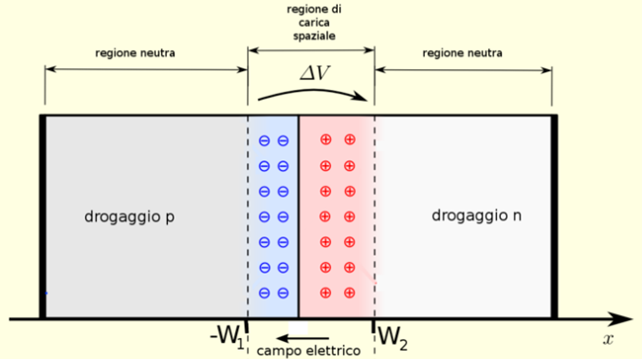
\includegraphics[width=0.55\linewidth]{Immagini/giunz. pn.png}
    \caption{diagramma giunzione P-N.}
    \label{fig: giunz. pn}
\end{figure}

La conseguenza della creazione della zona di svuotamento è la creazione di un campo elettrico causato dagli ioni negativi e positivi a seguito dell'annichilamento degli elettroni con le lacune. Il processo non continua all'infinito ma termina quando si raggiunge una situazione di equilibrio quando la zona di svuotamento è troppo grande per permettere la diffusione di ulteriori elettroni. La differenza di potenziale che si osserva nella regione di svuotamento è chiamata potenziale di built-in. Indicando con $V_T$ la tensione termica, la sua espressione analitica è
\begin{equation}
    V_0=V_T\ln{\left(\frac{n_An_D}{n_i^2}\right)}.
\end{equation}
\begin{obs}
    A $T=\SI{300}{\K}$ con $n_A\approx n_D\approx\SI{e16}{\cm^{-3}}$ e $n_i=\SI{e10}{\cm^{-3}}$, la tensione built-in per il silicio è $V_0=\SI{0.7}{\V}$.
\end{obs}
Se una tensione elettrica positiva viene applicata al lato di tipo P, i portatori di carica positivi, le lacune, maggioritari in questa regione sono spinti verso la giunzione. Ugualmente, i portatori di carica maggioritari nel lato N, gli elettroni, vengono attratti dalla tensione positiva e quindi sono attratti verso la giunzione. Poiché si ha una abbondanza di portatori di carica presso quest'ultima, la corrente può scorrerci attraverso sotto l'azione di una sorgente, come una batteria. La zona di svuotamento si restringe all'aumentare della tensione esterna con un conseguente abbassamento del potenziale di built-in e aumento della corrente di diffusione. In questo caso la giunzione si dice polarizzata direttamente.
\begin{figure}[h]
    \centering
    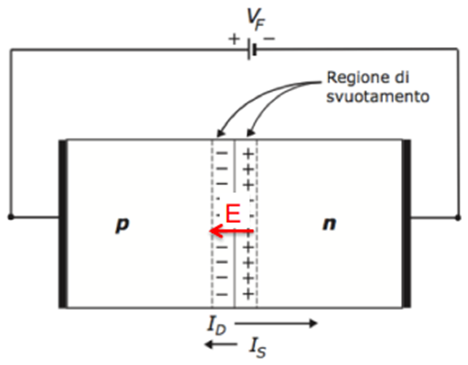
\includegraphics[width=0.5\linewidth]{Immagini/pol. dir. giunz. pn.png}
    \caption{diagramma polarizzazione diretta di una giunzione P-N.}
    \label{fig: pl. dir. pn}
\end{figure}

Se invece la polarizzazione della tensione viene invertita, le lacune e gli elettroni vengono allontanati dalla giunzione, lasciando una regione di silicio quasi non conduttore che non consente il flusso di corrente. La zona di svuotamento si allarga all'aumentare della tensione esterna con un conseguente innalzamento del potenziale di built-in e diminuzione della corrente di diffusione. Attraverso la giunzione passano però i minoritari che creano una piccolissima corrente $I_S$ detta di saturazione inversa. In questo caso la giunzione si dice polarizzata inversamente.
\begin{figure}[h]
    \centering
    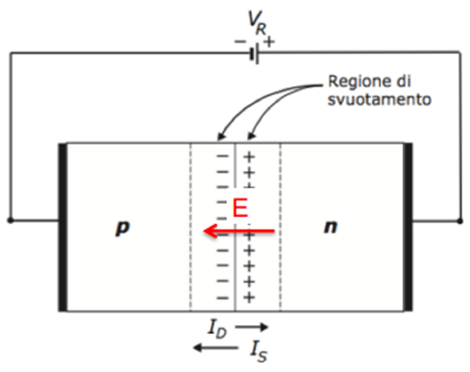
\includegraphics[width=0.5\linewidth]{Immagini/pol. inv. giunz. pn.png}
    \caption{diagramma polarizzazione inversa di una giunzione P-N.}
    \label{fig: pol. inv. on}
\end{figure}

\section{Diodo}
Un diodo è una giunzione P-N. L'andamento della caratteristica I-V di un diodo al silicio è descritto dalla legge di Shockley
\begin{equation}
    \label{eq: shockley}
    I(V)=I_S\left(e^{V/(\eta V_T)}-1\right),
\end{equation}
dove $\eta$ è il fattore di idealità, $V_T$ è la tensione termica e $I_S$ è la corrente di saturazione inversa, la quale è dovuta unicamente ai minoritari. All'aumentare della tensione ai capi del diodo si arriva ad un punto di rottura dei legami degli elettroni di valenza degli atomi di silicio. Macroscopicamente si osserva una scarica elettrica che brucia il diodo.
\begin{figure}[h]
    \centering
    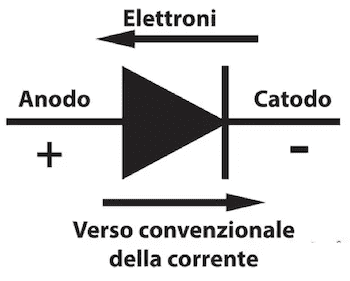
\includegraphics[width=0.3\linewidth]{Immagini/simbolo diodo.png}
    \caption{simbolo circuitale del diodo.}
    \label{fig: simbolo diodo}
\end{figure}

\'E possibile definire una resistenza dinamica del diodo che vale punto per punto derivando la tensione rispetto alla corrente
\begin{equation}
    r_d=\frac{dV}{dI}.
\end{equation}
Anche i LED sono diodi, i quali emettono luce al passaggio della corrente. Questo deriva dall'emissione di un fotone a seguito del salto energetico quantico effettuato dall'elettrone. Per i diodi LED è necessario aggiungere un termine ulteriore di resistenza alla legge di Shockley. Quindi, si ha
\begin{equation}
    \frac{I}{I_S}=e^{V/(\eta V_T)}-1\quad\therefore\quad\frac{V}{\eta V_T}=\ln{\left(\frac{I}{I_S}+1\right)}.
\end{equation}
Dunque, riarrangiando l'ultima relazione, si ottiene
\begin{equation}
    V(I)=\eta V_T\ln{\left(\frac{I}{I_S}+1\right)}+R_dI,
\end{equation}
dove il termine resistivo si è aggiunto solo dopo aver invertito l'equazione \eqref{eq: shockley} dato che, in caso contrario, si sarebbe ottenuta una relazione trascendente.

\paragraph{Modellizzazione di un diodo.} Un primo modello consiste nell'approssimare la curva di Shockley attraverso una resistenza dell'ordine di 10 M$\Omega$ e la combinazione in serie di un generatore di tensione di 0.7 V e una resistenza dell'ordine di 10 $\Omega$, rispettivamente per la polarizzazione inversa e per la polarizzazione diretta. 

Un secondo modello, più rozzo del primo, consiste nell'approssimare la polarizzazione inversa con un circuito aperto, mentre invece per la polarizzazione diretta si approssima la curva con un generatore di tensione ideale di 0.7 V. Essenzialmente il modello ci dice che il diodo sotto 0.7 V non conduce e sopra questa soglia conduce. 

Un terzo modello, molto semplice, per la polarizzazione inversa si approssima con un circuito aperto e per la polarizzazione diretta si approssima con un circuito chiuso. Essenzialmente in polarizzazione inversa il diodo non conduce, mentre in polarizzazione diretta conduce.

\section{Transistor}
Il transistor BJT (Bipolar Junction Transistor) è un componente elettronico a semiconduttore ampiamente utilizzato nei circuiti elettronici per la sua capacità di amplificare segnali o agire come interruttore. 
\begin{figure}[h]
    \centering
    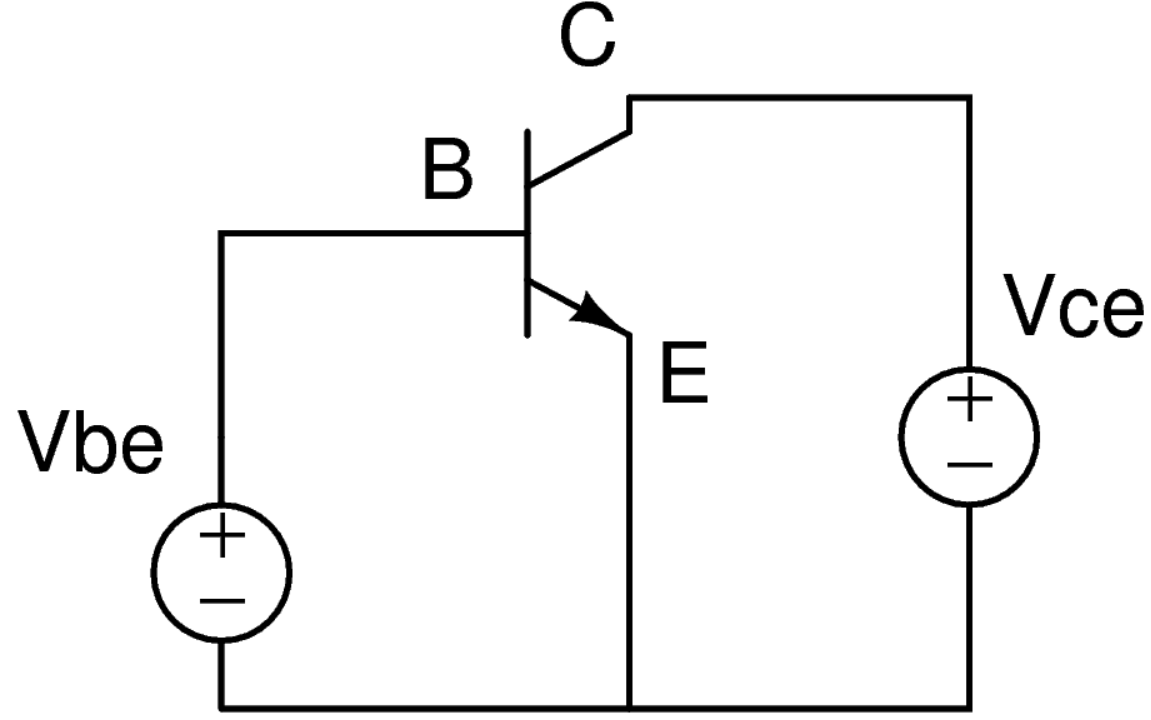
\includegraphics[width=0.4\linewidth]{Immagini/transistor npn.png}
    \caption{transistor BJT a giunzione NPN}
    \label{fig: trans. npn}
\end{figure}

È costituito da tre strati di materiale semiconduttore che formano due giunzioni PN: l'emettitore, la base e il collettore. Esistono due tipi di BJT: a giunzione NPN e a giunzione PNP. Il funzionamento del transistor si basa sul controllo della corrente che fluisce tra il collettore e l'emettitore attraverso una piccola corrente applicata alla base, permettendo di ottenere un guadagno di corrente. In particolare, gli strati componenti il transistor hanno caratteristiche e scopi diversi:
\begin{enumerate}
    \item emettitore: strato fortemente drogato, il cui scopo è emettere portatori di carica (elettroni in un NPN e lacune in un PNP) nella base.
    \item base: strato molto sottile e leggermente drogato, che separa l'emettitore dal collettore;
    \item collettore: strato moderatamente drogato, destinato a raccogliere i portatori di carica che attraversano la base.
\end{enumerate}
\begin{obs}
    Nel caso la base del transistor sia molto lunga la maggior parte degli elettroni non riesce ad arrivare al collettore, annichilendosi con le lacune nella base: il transistor si comporta come due diodi back-to-back.
\end{obs}

\paragraph{Funzionamento.} Il funzionamento del BJT (in regime normale) si basa sulle polarizzazioni delle giunzioni BE e BC. Infatti quando si applica alla giunzione BE una tensione positiva (polarizzazione diretta: base positiva rispetto a emettitore), la barriera di potenziale si riduce, permettendo agli elettroni di fluire dall'emettitore alla base. Dall'altra parte, alla giunzione BC è applicata una tensione ``negativa'' (polarizzazione inversa: collettore positivo rispetto alla base), la quale tende a bloccare il passaggio di cariche, lasciando però passare gli elettroni che attraversano la base senza annichilirsi. Quindi quando la giunzione BE è polarizzata direttamente, una corrente $I_B$ relativamente piccola fluisce dalla base. Quest'ultima provoca l'iniezione di elettroni dall'emettitore nella base. Dato che quest'ultima è molto sottile e leggermente drogata, la maggior parte degli elettroni la attraversa senza annichilirsi e arriva alla giunzione BC, polarizzata inversamente. Ora gli elettroni vengono attratti dal collettore, creando una corrente $I_C$ nel circuito di collettore. Quest'ultima è quindi molto più grande della corrente della base $I_B$ per cui vale $I_C\approx \beta_f I_B$, dove $\beta_f$ è il fattore di amplificazione del transistor. Variando pertanto la corrente $I_B$ si può controllare la corrente $I_C$, principio su quale si base il funzionamento del transistor BJT. In sintesi, l'obiettivo è di avere la maggior parte degli elettroni andare dall'emettitore al collettore; per farlo si droga pesantemente l'emettitore in modo da avere $I_C\approx I_E$, dove $I_C=\alpha_f I_E$, con $\alpha_f\approx0.9-0.99$. Applicando l'equazione \eqref{eq: sumI=0} si ha $I_E=I_B+I_C$, da cui
\begin{equation}
    I_C=\frac{\alpha_f}{1-\alpha_f}I_B=\beta_f I_B,\quad\beta_f\approx200.
\end{equation}

Ora l'obiettivo consiste nell'ottenere una tensione $V_{CE}$ che non modifichi la corrente $I_C$ (modificare $V_{CE}$ implica modificare l'area di svuotamento). Quindi, si droga il collettore meno della base in modo che lo svuotamento si estenda più verso il primo e che le cariche continuino a muoversi.

\paragraph{Tensione di built-in.} Quando un semiconduttore di tipo P e uno di tipo N vengono messi in contatto, gli elettroni del materiale di tipo N tendono a diffondersi nel materiale di tipo P e viceversa, le lacune del materiale P tendono a diffondersi nel materiale N. Questo movimento di cariche crea una regione di svuotamento nella giunzione, dove non ci sono più portatori mobili, lasciando dietro di sé solo cariche fisse (ioni positivi nel lato N e negativi nel lato P). Questa separazione di cariche genera un campo elettrico che si oppone al movimento ulteriore delle cariche, stabilendo una tensione di equilibrio detta di built-in. Quest'ultima ha due principali implicazioni:
\begin{enumerate}
    \item per polarizzare direttamente la giunzione BE (regime normale), è necessario applicare una tensione esterna superiore alla tensione di built-in. Questa tensione supera la barriera di potenziale della giunzione e permette il flusso di cariche attraverso di essa;
    \item anche la giunzione BC ha una tensione di built-in. Tuttavia, nel regime normale, questa giunzione è polarizzata inversamente, quindi la tensione esterna applicata è generalmente più alta e opposta rispetto alla tensione di built-in.
\end{enumerate}

\subsection{Regimi di funzionamento} 
Il transistor BJT può operare in diversi regimi. Questi si distinguono a seconda della polarizzazione delle giunzioni BE e BC.

\paragraph{Regime di saturazione.} In questo regime il transistor è completamente ``acceso'', permettendo il passaggio di una corrente massima dal collettore all'emettitore (agisce come interruttore chiuso). Le giunzione BE e BC sono polarizzate direttamente, mentre la tensione $V_{CE}$ è molto bassa, tipicamente intorno a $\SI{0.2}{\V}$ per un transistor NPN (in prima approssimazione si può porre $V_{CE}=0$). Le condizioni per questo regime sono
\begin{equation}
    V_{CE}=0,\quad V_{BE}>V_{\gamma},\quad V_{BC}>V_{\gamma,BC},
\end{equation}
dove $V_\gamma$ e $V_{\gamma,BC}$ sono le tensioni di soglia rispettive.

\paragraph{Regime normale.} In questo regime il transistor funziona come amplificatore, infatti vale la relazione $I_C=\beta_f I_B$. La giunzione BE è polarizzata direttamente, mentre la giunzione BC inversamente. Invece, la tensione $V_{CE}$ è compresa i valori della tensione di saturazione e di interdizione, mentre si ha $V_{BE}=V_{\gamma}=0.7$ V e $V_{\gamma}\neq V_{\gamma,BC}$ per via del diverso drogaggio di base e collettore, per cui la condizione per questo regime è
\begin{equation}
    V_{CE}=V_{BE}-V_{BC}>V_{\gamma}-V_{\gamma,BC}=V_{CE,sat}=0.3\approx0.
\end{equation}
Lo si può modellare con un generatore di corrente $I_C$, come in figura \ref{fig: trans. norm.}.
\begin{figure}[h]
            \centering
            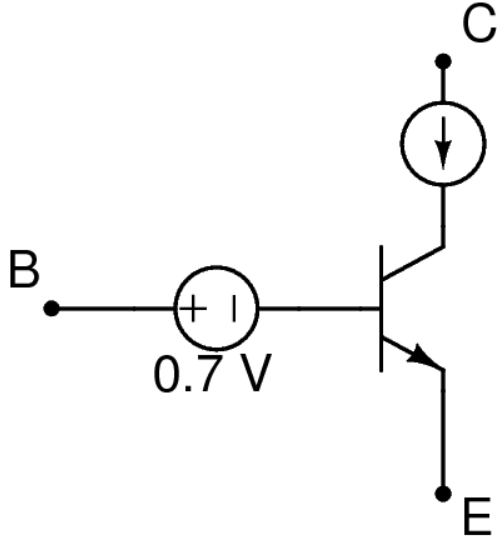
\includegraphics[width=0.25\linewidth]{Immagini/trans. norm..png}
            \caption{modellizzazione transistor in regime normale.}
            \label{fig: trans. norm.}
        \end{figure}

\paragraph{Regime di interdizione.} In questo regime, il transistor è completamente ``spento'', non scorre corrente tra collettore ed emettitore $I_C\approx0$ poiché $I_B\approx0$ (agisce come un interruttore aperto). Le giunzioni BE e BC sono polarizzate inversamente, mentre la tensione $V_{CE}$ è massima, paragonabile a $V_{CC}$ Le condizioni per questo regime sono
\begin{equation}
    V_{BE}<V_{\gamma},\quad V_{BC}<V_{\gamma,BC}.
\end{equation}

\paragraph{Regime di inverso.} In questo regime, la giunzione BE è polarizzata inversamente, mentre la giunzione BC direttamente. Inoltre, la corrente di emettitore diventa maggiore di $I_C$, con un guadagno di corrente molto ridotto rispetto al regime normale.
\begin{table}[H]
    \centering
    \begin{tabular}{|c|c|c|}
        \hline
        \textbf{BE} & \textbf{BC} & \textbf{Regime} \\ \hline
        inversa & inversa & interdizione \\ \hline
        diretta & inversa & normale \\ \hline
        diretta & diretta & saturazione \\ \hline
        inversa & diretta & inverso \\ \hline
    \end{tabular}
    \caption{sintesi delle condizioni dei regimi di funzionamento.}
    \label{tab: reg. funz. trans.}
\end{table}
\begin{table}[H]
  \centering
  \begin{tabular}{|c|c|c|c|}
    \hline
    \textbf{Interdizione} & \textbf{Normale} & \textbf{Saturazione} \\ 
    \hline
    0 & $< I_C <$ & $I_{C,max} = V_{CC}/R_C$ \\ 
    \hline
    $V_{CC}$ & $> V_{CE} >$ & $V_{CE,sat} \approx 0\,V$ \\ 
    \hline
  \end{tabular}
  \caption{sintesi dei limiti di funzionamento.}
  \label{tab: lim. funz. trans.}
\end{table}
\begin{ex}
    Si consideri il circuito in figura \ref{fig: trans. ex.}. Per restare in regime normale si deve avere $V_{CE}>0$, da cui si deduce un limite su $I_C$ e $I_B$. 
        \begin{figure}[H]
        \centering
        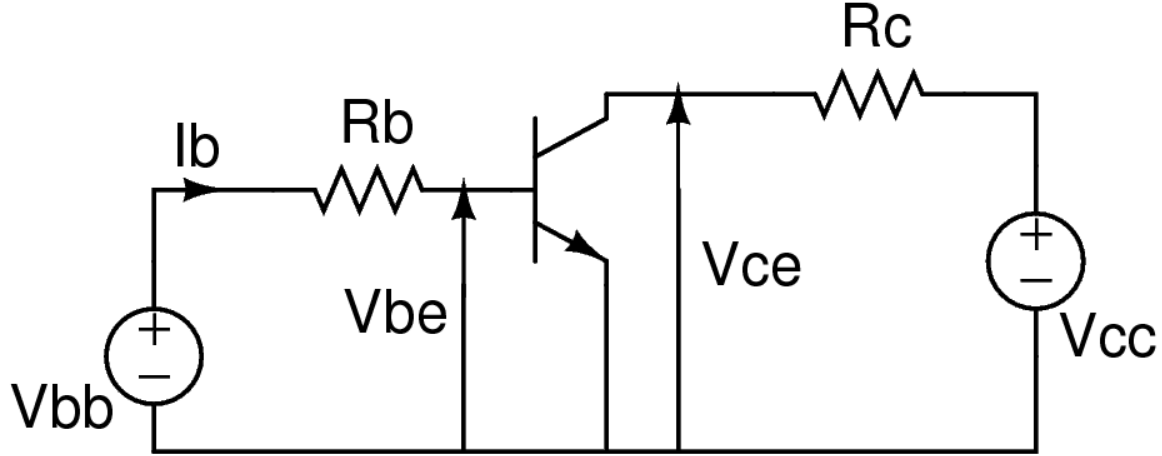
\includegraphics[width=0.6\linewidth]{Immagini/trans. ex..png}
        \caption{circuito con transistor BJT}
        \label{fig: trans. ex.}
    \end{figure}
    
    Applicando l'equazione \eqref{eq: sumV=0} si ottiene
    \begin{equation}
        I_B=\frac{V_{BB}-0.7}{R_B},
    \end{equation}
    che deve soddisfare la condizione $I_B>0$ affinché si abbia regime normale. Da
    \begin{equation}
        V_{CE}=V_{CC}-I_CR_C=V_{CC}-\beta I_BR_C,
    \end{equation}
    si ricava il limite su $I_C$ per cui si ha regime di saturazione quando
    \begin{equation}
        I_{C,max}=\frac{V_{CC}}{R_C}.
    \end{equation}
    Il transistor è in interdizione quando $I_B=I_C=0$ e $V_{CE}=V_{CC}$.
\end{ex}
\chapter{Ottica geometrica e Fisica moderna}
L'Ottica geometrica studia la propagazione della luce assumendo che si muova in linee rette. Analizza la formazione delle immagini attraverso strumenti ottici come specchi e lenti, basandosi sui fenomeni della riflessione e della rifrazione per spiegare come la luce interagisce con gli oggetti.
\begin{defn}[oggetto]
    L'oggetto per uno strumento ottico è un corpo, puntiforme ed esteso, che emette luce direttamente o diffonde la luce emessa da un altro corpo.
\end{defn}
\begin{defn}[immagine]
    L'immagine è la figura che si crea dai raggi luminosi convergenti dopo aver attraversato lo strumento. L'immagine può essere:
    \begin{enumerate}
        \item reale se i raggi si incontrano fisicamente nei suoi punti;
        \item virtuale se per essa passano i prolungamenti dei raggi, ma non i raggi stessi.
    \end{enumerate}
\end{defn}
\begin{defn}[punti coniugati]
    I punti coniugati sono le posizioni di un punto dell'oggetto e del rispettivo punto dell'immagine.
\end{defn}
\begin{defn}[stigmatismo]
    Se i raggi uscenti da un punto dell'oggetto si incontrano in un solo punto dell'immagine lo strumento è definito stigmatico.
\end{defn}
Lo stigmatismo, condizione essenziale per un a buona definizione dell'immagine, è difficile da ottenere: l'immagine di un punto è quasi sempre estesa, cioè non puntiforme. Nell'ottica geometrica si usa considerare superfici speculari o rifrattive di forma sferica. In queste condizioni, solo se si assumono fasci di raggi di piccola apertura e parassiali, cioè vicini all'asse ottico e formanti con questo angoli molto piccoli, è possibile raggiungere con buona approssimazione una situazione di stigmatismo. Queste approssimazioni sono raccolte sotto il nome di approssimazioni di Gauss.
\begin{axiom}[approssimazioni di Gauss]\hfill
    \begin{enumerate}
        \item Il fascio di raggi che incidono sul sistema ottico deve avere piccola apertura rispetto alle dimensioni del sistema.
        \item I raggi devono essere ragionevolmente parassiali, ovvero avere una piccola inclinazione rispetto all'asse ottico
    \end{enumerate}
\end{axiom}
\begin{defn}[specchi]
    Superfici che la luce incontra su cui può avvenire solo riflessione
\end{defn}
\begin{defn}[diottri]
    Superfici che la luce incontra su cui può avvenire solo trasmissione da un mezzo all'altro.
\end{defn}
Nella costruzione delle immagini negli specchi, nei diottri e nelle lenti è conveniente adottare alcune convenzioni sui segni delle distanze che permettono di trattare tutti i casi senza ambiguità. Allo scopo di semplificare la trattazione degli argomenti è conveniente adottare una convenzione diversa per gli specchi e per i diottri e le lenti.
\begin{axiom}[convenzioni specchi]\hfill
    \begin{enumerate}
        \item La luce proviene sempre da sinistra.
        \item La distanza $p$ di un oggetto P dal vertice V è positiva se l'oggetto si trova a sinistra del vertice, negativa se l'oggetto è a destra di V.
        \item La distanza $q$ dell'immagine Q dal vertice V è negativa se l'oggetto si trova a destra del vertice, positiva se l'oggetto è a sinistra di V.
        \item Il raggio di curvatura $R$ della superficie sferica è negativo se il centro di curvatura si trova a destra di V, positivo se il centro di curvatura si trova a sinistra di V.
        \item Le distanze $y$ dall'asse sono positive per punti al di sopra dell'asse, negative per punti al di sotto, sia per oggetti che per le immagini.
    \end{enumerate}
\end{axiom}
\begin{axiom}[convenzioni diottri e lenti]\hfill
    \begin{enumerate}
        \item La luce proviene sempre da sinistra.
        \item La distanza $p$ di un oggetto P dal vertice V è positiva se l'oggetto si trova a sinistra del vertice, negativa se l'oggetto è a destra di V.
        \item La distanza $q$ dell'immagine Q dal vertice V è positiva se l'oggetto si trova a destra del vertice, negativa se l'oggetto è a sinistra di V.
        \item Il raggio di curvatura $R$ della superficie sferica è positivo se il centro di curvatura si trova a destra di V, negativo se il centro di curvatura si trova a sinistra di V.
        \item Le distanze $y$ dall'asse sono positive per punti al di sopra dell'asse, negative per punti al di sotto, sia per oggetti che per le immagini.
    \end{enumerate}
\end{axiom}
La propagazione dei raggi luminosi avviene tipicamente attraverso mezzi diversi. L'insieme dei mezzi e delle superfici che li separano definisce un sistema ottico. Un sistema ottico può essere composto da diversi elementi posti in successione lungo il percorso dei raggi luminosi.
\begin{figure}[H]
    \centering
    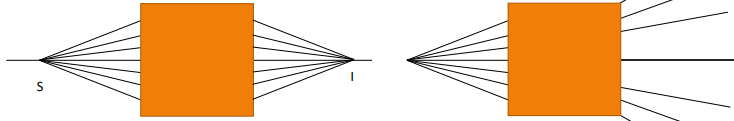
\includegraphics[width=0.75\linewidth]{Immagini ottica/sistemi conv. e div..png}
    \caption{diagramma di un sistema convergente e divergente.}
    \label{fig: sist. conv. e div.}
\end{figure}

In un sistema convergente, i raggi provenienti da sorgente puntiforme convergono in un punto detto immagine. Invece, in un sistema divergente, i raggi divergono e non si forma un'immagine.
\begin{figure}[h]
    \centering
    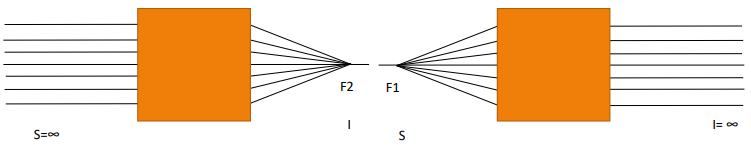
\includegraphics[width=0.75\linewidth]{Immagini ottica/fuochi sist. conv.png}
    \caption{diagramma fuochi di un sistema convergente.}
    \label{fig: fuochi sist. conv.}
\end{figure}

In un sistema convergente sono presenti due fuochi. Il primo fuoco è il punto da cui provengono i raggi la cui immagini si forma all'infinito; il secondo fuoco è il punto in cui i raggi provenienti dall'infinito convergono. Nel caso del secondo fuoco, i raggi possono essere prolungati all'indietro verso la direzione di provenienza. L'immagine si crea quindi a sinistra del sistema ottico, nello spazio degli oggetti. L'immagine che si forma è virtuale.

\section{Diottro sferico}
Un diottro sferico è un sistema ottico costituito da due mezzi omogenei (di indice di rifrazione $n_1$ e $n_2$ diversi, tali che $n_1<n_2$), trasparenti e isotropi, separati da una superficie sferica di raggio $R$. L'asse ottico interseca la superficie sferica nel punto V, riferimento per la misura delle distanze.
\begin{figure}[h]
    \centering
    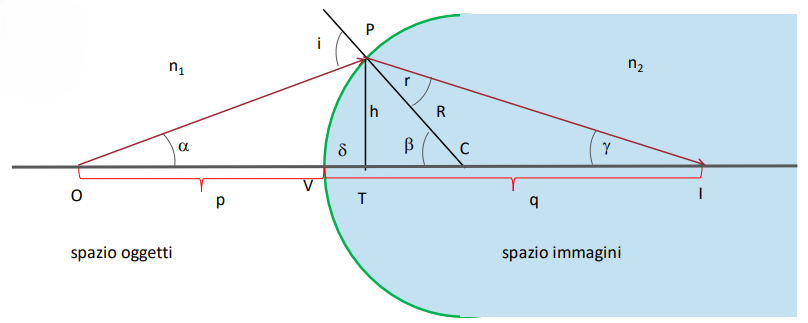
\includegraphics[width=0.8\linewidth]{Immagini ottica/diottro sferico.png}
    \caption{diagramma di un diottro sferico.}
    \label{fig: diottro sferico}
\end{figure}

Per costruire l'immagine si consideri un generico raggio luminoso emesso dalla sorgente O con angolo $\alpha$ rispetto all'asse ottico; esso viene rifratto nel punto P intersecando l'asse ottico nel punto I. Si applica quindi la secondo legge di Snell nel punto P scrivendo 
\begin{equation}
    \label{eq: snell diottro in P}
    n_1\sin{i}=n_2\sin{r}.
\end{equation}
Considerando le proprietà degli angoli si ricava che
\begin{equation}
    \begin{cases}
        \label{eq: angoli i e r diottro}
        i=\alpha+\beta \\
        \beta=r-\gamma\Rightarrow r=\beta-\gamma
    \end{cases}.
\end{equation}
Sostituendo le relazioni del sistema \eqref{eq: angoli i e r diottro} nell'equazione \eqref{eq: snell diottro in P} si ha
\begin{equation}
    \label{eq: snell diottro in P 2}
    n_1\sin{(\alpha+\beta)}=n_2\sin{(\beta-\gamma)}.
\end{equation}
Applicando ora le condizioni dell'approssimazione di Gauss degli assi parassiali si può scrivere l'equazione \eqref{eq: snell diottro in P 2} come
\begin{equation}
    n_1(\alpha+\beta)=n_2(\beta-\gamma)\quad\therefore\quad n_1\alpha +n_2\gamma=\beta(n_2-n_1).
\end{equation}
A questo punto si può applicare ancora l'approssimazione di Gauss, considerando che gli angoli possono essere approssimati alle tangenti
\begin{equation}
\tan{\beta}=\dfrac{h}{R-\delta},\quad\tan{\gamma}=\dfrac{h}{q-\delta},\quad\tan{\alpha}=\dfrac{h}{p+\delta},
\end{equation}
ottenendo pertanto
\begin{equation}
    \label{eq: pre-equazione del diottro}
    \frac{n_1}{p-\delta}+\frac{n_2}{q-\delta}=\frac{n_2-n_1}{R-\delta}.
\end{equation}
Se si assume che il segmento $\delta$ sia trascurabile rispetto a $p$, $q$ e $R$ l'equazione \eqref{eq: pre-equazione del diottro} diventa l'equazione del diottro
\begin{equation}
    \label{eq: equazione del diottro}
    \frac{n_1}{p}+\frac{n_2}{q}=\frac{n_2-n_1}{R}.
\end{equation}
L'equazione del diottro fornisce una relazione tra la posizione $p$ della sorgente e la posizione $q$ dell'immagine indipendentemente dal valore di $\alpha$. In approssimazione di Gauss, il diottro trasforma fasci omocentrici in fasci rifratti omocentrici. L'equazione \eqref{eq: equazione del diottro} è detta anche equazione di Cartesio e i punti di coordinate $p$ e $q$ che la soddisfano sono detti punti coniugati rispetto al diottro.

\paragraph{Fuochi.} Se la posizione $p$ della sorgente tende all'infinito, l'immagine si trova in un punto $F_2$, posto a distanza $f_2$ dal diottro sferico detto secondo fuoco. Se l'immagine si forma a distanza infinita, l'oggetto si trova in un punto $F_1$, detto primo fuoco, a distanza $f_1$ dal diottro e i raggi uscenti da $F_1$ si rifrangono parallelamente all'asse ottico. Dall'equazione \eqref{eq: equazione del diottro} si ricavano i valori di $f_1$ e $f_2$ come
\begin{equation}
    \begin{cases}
        f_2=\lim_{p\to\infty}{q}=R\dfrac{n_2}{n_2-n_1} \\[2ex]
        f_1=\lim_{q\to\infty}{p}=R\dfrac{n_1}{n_2-n_1}
    \end{cases}.
\end{equation}
Dunque, l'equazione \eqref{eq: equazione del diottro} può essere riscritta come
\begin{equation}
    \frac{f_1}{p}+\frac{f_2}{q}=1,
\end{equation}
da cui si ricava che se l'oggetto è posto tra il primo punto focale e l'infinito ($p> f_1$), esso fornisce un'immagine reale, mentre fornisce un'immagine virtuale quando è posta tra la superficie del diottro e il primo fuoco ($p< f_1$).
\section{Lenti sottili}
Due superfici diottriche aventi lo stesso asse individuano tre regioni distinte: la luce proveniente da sinistra si propaga nel primo mezzo avente indice di rifrazione $n_1$, viene trasmessa dal primo diottro e attraversa il mezzo con indice di rifrazione $n_2$ e infine, dopo la trasmissione al secondo diottro, si propaga nel mezzo con indice di rifrazione $n_3$. Le superfici diottriche possono essere piane o sferiche, convergenti o divergenti. Il mezzo avente indice di rifrazione $n_2$ si chiama lente semplice. Si trattano in particolare casi in cui $n_1=n_3$ e le lenti sono sottili, ovvero con superfici diottriche molto vicine.
\begin{figure}[h]
    \centering
    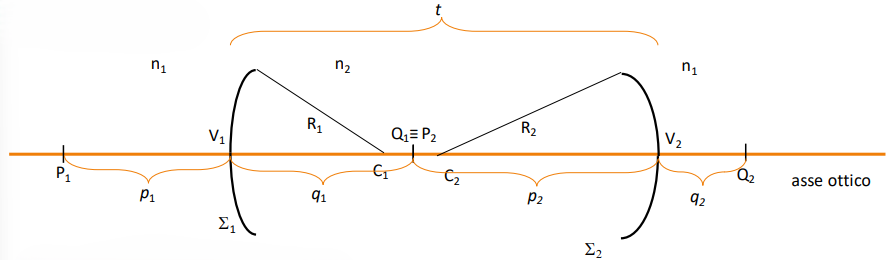
\includegraphics[width=0.95\linewidth]{Immagini ottica/lenti sottili.png}
    \caption{diagramma di una lente sottile.}
    \label{fig: lente sottile}
\end{figure}

Le equazioni dei due diottri, assumendo che l'immagine generata dal primo diventi oggetto del secondo, sono
\begin{equation}
    \begin{cases}
        \dfrac{n_1}{p_1}+\dfrac{n_2}{q_1}=\dfrac{n_2-n_1}{R_1} \\[2ex]
        \dfrac{n_2}{t-q_1}+\dfrac{n_1}{q_2}=\dfrac{n_1-n_2}{R_2},
    \end{cases}
\end{equation}
dove per costruzione si ha $p_2=t-q_1$. Supponendo che $t$ sia trascurabile rispetto alle altre distanze e sommando membro a membro si ottiene
\begin{equation}
    \frac{1}{p_1}+\frac{1}{q_2}=\frac{n_2-n_1}{n_1}\left(\frac{1}{R_1}-\frac{1}{R_2}\right).
\end{equation}
Definendo quindi $p_1=p$ come la distanza dell'oggetto e $q_2=q$ come la distanza immagine si ottiene
\begin{equation}
    \label{eq: eq. costruttore lenti}
    \frac{1}{p}+\frac{1}{q}=\frac{n_2-n_1}{n_1}\left(\frac{1}{R_1}-\frac{1}{R_2}\right)=\dfrac{1}{f},
\end{equation}
dove $f_1=f_2=f$.
L'equazione \eqref{eq: eq. costruttore lenti} permette di definire i fuochi di una lente sottile
\begin{equation}
    \begin{cases}
        f_2=\lim_{p\to\infty}{q}=\dfrac{1}{f_2}=\dfrac{n_2-n_1}{n_1}\left(\dfrac{1}{R_1}-\dfrac{1}{R_2}\right) \\[2ex]
        f_1=\lim_{q\to\infty}{p}=\dfrac{1}{f_1}=\dfrac{n_2-n_1}{n_1}\left(\dfrac{1}{R_1}-\dfrac{1}{R_2}\right)
    \end{cases}
\end{equation}
Inoltre, dall'equazione \eqref{eq: eq. costruttore lenti} si ricava la legge dei punti coniugati
\begin{equation}
    \label{eq: legge dei punti coniugati}
    \frac{1}{p}+\frac{1}{q}=\frac{1}{f}.
\end{equation}
\begin{defn}[potere diottrico]
    Il potere diottrico $P$ di una lente è l'inverso della distanza focale $f$ espressa in metri. La sua unità di misura è la diottria.
\end{defn}

\paragraph{Sistemi di lenti sottili.} Si considerino due lenti sottili poste in successione di focali rispettivamente $f_1$ e $f_2$. Assumendo che l'immagine creata dalla prima lente diventi oggetto della seconda e ricordando che 
\begin{equation}
    \begin{cases}
    \label{eq: sistema lenti a contatto}
        \dfrac{1}{f_1}=\dfrac{1}{p_1}+\dfrac{1}{q_1} \\[2ex]
        \dfrac{1}{f_2}=\dfrac{1}{p_2}+\dfrac{1}{q_2},
    \end{cases}
\end{equation}
dove $p_2=d-q_1$. Sommando le equazioni del sistema \eqref{eq: sistema lenti a contatto} si trova
\begin{equation}
    \label{eq: eq: somma sistema lenti a contatto}
    \dfrac{1}{f_1}+\dfrac{1}{f_2}=\dfrac{1}{p_1}+\dfrac{1}{q_1}+\dfrac{1}{d-q_1}+\dfrac{1}{q_2}.
\end{equation}
Se $d=0$, ovvero se le lenti sono a contatto, l'equazione \eqref{eq: eq: somma sistema lenti a contatto} diventa
\begin{equation}
    \dfrac{1}{f_1}+\dfrac{1}{f_2}=\dfrac{1}{p}+\dfrac{1}{q},
\end{equation}
dove $p$ e $q$ rappresentano la distanza
oggetto e immagine del sistema. Si definisce pertanto la focale $f$ del sistema di lenti a contatto per cui vale
\begin{equation}
    \label{eq: focale sistema lenti a contatto}
    \frac{1}{f}=\dfrac{1}{f_1}+\dfrac{1}{f_2}.
\end{equation}

\paragraph{Ingrandimento.} Si consideri una lente sottile. Come mostrato in figura \ref{fig: ingrandimento}, indicando con $V$ il centro della lente sottile, dato che il triangolo formato da $h_o$, la distanza oggetto-V e il raggio passante per il centro, è simile al triangolo formato da $h_i$, la distanza immagine-V e il medesimo raggio, si può scrivere
\begin{equation}
    \label{eq: ingrandimento}
    \frac{h_i}{h_o}=\frac{-q}{p}=G,
\end{equation}
dove $G$ è appunto il coefficiente di ingrandimento. Se $G>0$, allora l'immagine è dritta rispetto all'oggetto, mentre se $G<0$ l'immagine risulta capovolta.
\begin{figure}[h]
    \centering
    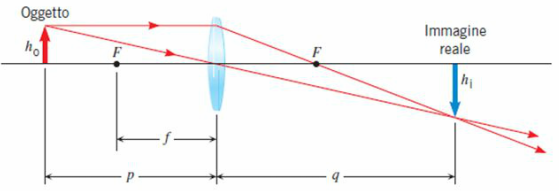
\includegraphics[width=0.65\linewidth]{Immagini ottica/ingrandimento.png}
    \caption{diagramma per ingrandimento di una lente sottile.}
    \label{fig: ingrandimento}
\end{figure}

\section{Aberrazioni}
\paragraph{Cromatismo.} Uno dei difetti ottici più semplici da riconoscere è l'aberrazione cromatica. Gli oggetti luminosi presentano aloni colorati più o meno diffusi. I colori più probabili da osservare sono il rosso e il blu, l'uno intra e l'altro extrafocale. Il problema nasce dall'impossibilità per una lente di mettere a fuoco tutte le lunghezze d'onda nello stesso piano focale per via della dispersione che la luce subisce attraversando materiali di densità ottica diversa. In pratica quando si fa il fuoco con un rifrattore acromatico di fatto si fa il fuoco nel verde sacrificando il rosso e il blu che finiscono sfuocati. Per correggere questo difetto ottico si usano i “doppietti acromatici”, ossia coppie di lenti convergente-divergente opportunamente lavorate.

\paragraph{Sfericità.} Quando dei raggi paralleli all'asse ottico incidono su una lente con superfici sferiche, solo i raggi parassiali passano per il fuoco parassiale $F$. Invece, i raggi più lontani dall'asse vengono deviati in punti più distanti rispetto ad $F$, mentre quelli più vicini all'asse vengono deviati in punti antecedenti $F$, come mostrato in figura \ref{fig: sfericità}. Questo effetto prende il nome di aberrazione sferica. A causa di questa aberrazione, l'immagine di un punto luminoso non risulta essere ancora un punto, ma una macchia luminosa di forma circolare, spesso circondata da un alone di luce. Tra tutti i punti lungo l'asse, ce n'è uno in cui il diametro di questa macchia è minimo, detto cerchio di minima confusione.
\begin{figure}[h]
    \centering
    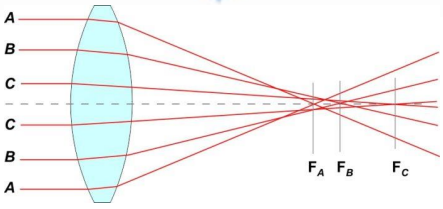
\includegraphics[width=0.5\linewidth]{Immagini ottica/sfericità.png}
    \caption{effetto della sfericità.}
    \label{fig: sfericità}
\end{figure}

\paragraph{Coma.} Questo difetto ottico avviene quando l'oggetto è lontano dall'asse ottico e i raggi sono tra di loro paralleli, ma inclinati rispetto all'asse della lente. Quando tali raggi incidenti attraversano la lente lontano dall'asse, i raggi rifratti non si incontrano tutti nello stesso punto, poiché la superficie della lente può essere approssimata con un piano solo nella zona parassiale. Di conseguenza, a seconda della distanza del raggio dal centro della lente la corrispondente immagine sarà un cerchio di raggio diverso e diversa distanza dall'asse. Per correggere questo difetto ottico si deve impiegare un diaframma in una posizione tale da limitare l'area della lente su cui i raggi obliqui sono incidenti.

\paragraph{Astigmatismo.} Questo difetto ottico avviene quando l'oggetto è vicino e fuori asse. Considerando un singolo punto dell'oggetto e seguendo il percorso dei raggi sul piano tangenziale e su quello sagittale:
\begin{itemize}
    \item i fasci di luce che incidono lungo il meridiano tangenziale AA' convergeranno nel punto T, detto immagine primaria;
    \item i fasci di luce che incidono lungo il meridiano sagittale BB' focalizzano nel punto S, detto immagine secondaria.
\end{itemize}
Nel punto T si trova il fuoco dei raggi tangenziali. I fasci sagittali non saranno ancora a fuoco, si vede una linea detta ``focalina'' o immagine tangenziale. Invece, nel punto S si trova il fuoco dei raggi sagittali. Il fascio dei raggi tangenziali diverge. Anche qui si vede un'immagine della focalina sagittale. La distanza tra le focaline è detta intervallo di Sturm. Quindi, la miglior immagine del punto P si può vedere a metà tra T e S ed è detto cerchio di minima confusione. Per correggere questo difetto ottico si devono usare lenti cilindriche; i sistemi corretti si dicono sistemi anastigmatici.
\begin{figure}[h]
    \centering
    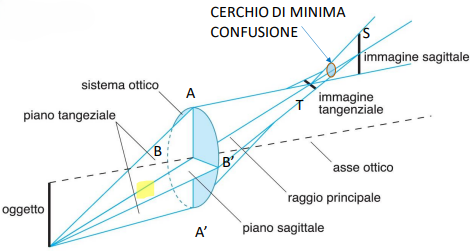
\includegraphics[width=0.7\linewidth]{Immagini ottica/astigmatismo.png}
    \caption{effetto dell'astigmatismo.}
    \label{fig: astigmatismo}
\end{figure}

\paragraph{Distorsioni.} Questo difetto ottico riguarda l'aberrazione della forma dell'immagine di un oggetto esteso dovuta al fatto che l'ingrandimento $G$ dipende dalla distanza del punto oggetto dall'asse $d$, si presentano due casi:
\begin{enumerate}
    \item se $G$ aumenta con $d$ si ha una distorsione a cuscinetto;
    \item se $G$ diminuisce con $d$ si ha una distorsione a barilotto.
\end{enumerate}
Per correggere questo difetto ottico si deve usare un sistema detto doppietto ortoscopico, formato da una coppia di lenti e un diaframma.
\begin{obs}
Per diaframma si intende una limitazione meccanica che riduce in una certa misura la quantità di radiazione che incide su un sistema ottico o che da esso viene trasmessa limitando l'apertura dei fasci. Il diaframma può essere posizionato all'ingresso del sistema, tra lenti all'interno di esso oppure in uscita.
\end{obs}

\section{Banco ottico}
Le ipotesi consistono nell'assumere che il sistema sia un sistema ottico centrato e che valgano le approssimazioni di Gauss. L'esperienza si articola in due parti contraddistinte da due obiettivi differenti: determinare la distanza focale tramite l'equazione \eqref{eq: legge dei punti coniugati} di una lente convergente e di un'altra divergente; verificare la legge dell'ingrandimento tramite l'equazione \eqref{eq: ingrandimento}.
\begin{figure}[h]
    \centering
    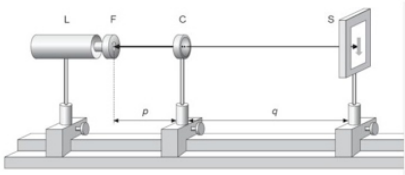
\includegraphics[width=0.7\linewidth]{Immagini ottica/apparato banco ottico.png}
    \caption{banco ottico.}
    \label{fig: banco ottico}
\end{figure}

Per determinare la focale della lente convergente e di quella divergente, i passi da seguire sono:
\begin{enumerate}
    \item lasciare fissa la distanza oggetto-lente $p$ e di cercare ripetutamente la posizione dello schermo che mette a fuoco l'immagine, variando la distanza lente-schermo $q$. Eseguire un numero di misurazioni tale che sia possibile valutare la distribuzione di $q$. Ripetere l'esercizio dopo aver ruotato la lente di 180°. Si valuti la compatibilità statistica delle distanze focali prima e dopo la rotazione della lente. Si facciano le considerazioni del caso riguardo alle distribuzioni ottenute. Si valuti la lunghezza focale della lente;
    \item variare alcune volte la distanza oggetto-lente $p$. Per ogni valore di $p$, si cerchi ripetutamente il valore di $q$ per cui l'immagine è a fuoco sullo schermo. Riportare le misure nel piano avente $1/p$ sulle ascisse e $1/q$ sulle ordinate. Eseguire un fit lineare ed estrarne la lunghezza focale;
    \item con lo stesso metodo, si misuri la lunghezza focale di una lente divergente (lunghezza focale negativa). Occorre combinarla con una lente convergente in modo che la focale risultante sia positiva. In particolare, per determinare la focale $f_{div}$ si deve usare la formula
    \begin{equation}
            \frac{1}{f_{sist}}=\frac{1}{f_{conv}}+\frac{1}{f_{div}}.
        \end{equation}
    \end{enumerate}
Per verificare la legge dell'ingrandimento ricavata in \eqref{eq: ingrandimento}, i passi da seguire sono:
\begin{enumerate}
    \item si misura la lunghezza di un particolare dell'immagine;
    \item si misurano diversi valori di $p$ e $q$;
    \item per ogni coppia di dati si misura la lunghezza dello stesso particolare sullo schermo;
    \item si confrontano i valori di $G$ ottenuti con la formula \eqref{eq: ingrandimento}.
\end{enumerate}

\section{Spettroscopio di Kirchhoff-Bunsen}
\paragraph{Prisma in deviazione minima.} Un modo molto semplice per disperdere la luce è tramite un prisma di vetro. Da considerazioni geometriche sugli angoli in figura \ref{fig: prisma} si trova che
\begin{equation}
    \begin{cases}
    \label{eq: sistema prisma}
        \theta=\pi-(i-r)-(i'-r') \\
        D=\pi-\theta=(i-r)+(i'-r') \\
        \beta+r=\gamma+r'=\pi/2 \\
        \alpha+\beta+\gamma=\pi \\
        \alpha=r+r'
    \end{cases}.
\end{equation}
\begin{figure}[H]
    \centering
    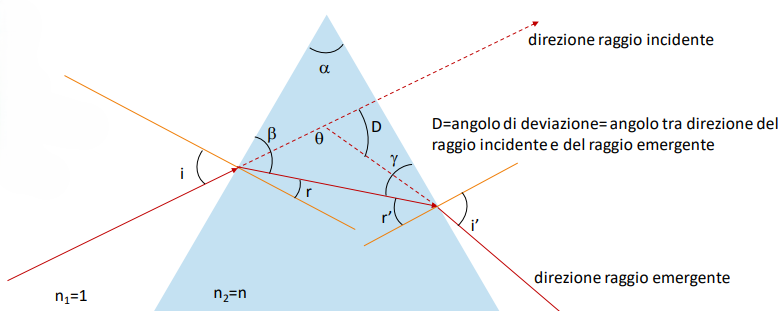
\includegraphics[width=0.85\linewidth]{Immagini ottica/Prisma.png}
    \caption{dispersione della luce tramite un prisma.}
    \label{fig: prisma}
\end{figure}

Ora considerando la penultima equazione del sistema \eqref{eq: sistema prisma} e sostituendo i valori di $\gamma$ e $\beta$ del sistema \eqref{eq: sistema prisma} si trova
\begin{equation}
    \label{eq: angolo alpha prisma}
    \alpha=\pi-\left(\frac{\pi}{2}-r\right)-\left(\frac{\pi}{2}-r'\right)=r+r'.
\end{equation}
Pertanto, si ha
\begin{equation}
    \label{eq: andolo d prisma}
    D=i+i'-\alpha=i+i'-r-r'.
\end{equation}
Ora partendo dalle equazioni \eqref{eq: angolo alpha prisma} e \eqref{eq: andolo d prisma} si può applicare la seconda legge di Snell per elaborare ulteriormente il risultato. Quindi, da
\begin{equation}
    \label{eq: sistema prisma 3}
    \begin{cases}
        \alpha=r+r' \\
        \sin{i}=n\sin{r} \\
        \sin{i'}=n\sin{r'}
    \end{cases},
\end{equation}
si ha 
\begin{equation}
    \sin{i'}=n\sin{r'}=n\sin{(\alpha-r)}=n(\sin{\alpha}\cos{r}-\cos{\alpha}\sin{r}),
\end{equation}
e sostituendo $\sin{r}$ con la prima equazione del sistema \eqref{eq: sistema prisma 3} si ottiene
\begin{equation}
    \begin{split}
    \label{eq: sin i' prisma}
    \sin{i'}&=n\left(\sin{\alpha}\sqrt{1-\frac{\sin^2{i}}{n^2}}-\cos{(\alpha)}\frac{\sin{i}}{n}\right) \\
    &=\sin{\alpha}\sqrt{n^2-\sin^2{i}}-\cos{\alpha}\sin{i}.
    \end{split}    
\end{equation}
Sostituendo quindi l'equazione \eqref{eq: sin i' prisma} nell'equazione \eqref{eq: andolo d prisma} si trova
\begin{equation}
    \label{eq: finale angolo d prisma}
    D=i-\alpha+\arcsin{\left(\sin{\alpha}\sqrt{n^2-\sin^2{i}}-\cos{\alpha}\sin{i}\right)}.
\end{equation}
L'equazione \eqref{eq: finale angolo d prisma} è molto utile per esigenze sperimentali in quanto l'unica grandezza da misurare per conoscere l'angolo di deviazione $D$ è l'angolo di incidenza $i$. Sempre da questa equazione si ricava
\begin{equation}
    \label{eq: indice rifrazione prisma generale}
    n=\sqrt{ \left(\sin{(D+\alpha-i)}+\sin{i}\cos{\alpha}\right)^2\frac{1}{\sin^2{\alpha}}+\sin^2{i}}
\end{equation}
Per semplificare la relazione \eqref{eq: indice rifrazione prisma generale}, si può cercare la condizione di incidenza per cui l'angolo $D$ è minimo. Per fare ciò si minimizza l'equazione \eqref{eq: andolo d prisma}. Si parte quindi dalle relazioni
\begin{equation}
    \begin{cases}
    \label{eq: sistema prisma min. dev.}
        D=i+i'-\alpha \\
        r'=\alpha-r \\
        \sin{i}=n\sin{r} \\
        n\sin{r'}=\sin{i'}
    \end{cases}.
\end{equation}
Differenziando il sistema \eqref{eq: sistema prisma min. dev.} si trova
\begin{equation}
    \begin{cases}
        dD=di+di' \\
        dr'=-dr \\
        \cos{(i)}di=n\cos{(r)}dr \\
        n\cos{(r')}dr'=\cos{(i')}di'
    \end{cases},
\end{equation}
da cui
\begin{equation}
    \begin{cases}
        di'=n\dfrac{\cos{r'}}{\cos{i'}}dr' \\[2ex]
        dr=\dfrac{1}{n}\dfrac{\cos{i}}{\cos{r}}di
    \end{cases}.
\end{equation}
Ora da $dr'=-dr$ si ha
\begin{equation}
    di'=n\frac{\cos{r'}}{\cos{i'}}dr'=-n\frac{\cos{r'}}{\cos{i'}}\frac{1}{n}\frac{\cos{i}}{\cos{r}}di=-\frac{\cos{r'}}{\cos{i'}}\frac{\cos{i}}{\cos{r}}di,
\end{equation}
che sostituito in $dD=di+di'$ restituisce
\begin{equation}
    \label{eq: dD/di}
    \frac{dD}{di}=1-\frac{\cos{r'}}{\cos{i'}}\frac{\cos{i}}{\cos{r}}.
\end{equation}
Minimizzando ora \eqref{eq: dD/di} ponendo $dD/di=0$, si ha la condizione
\begin{equation}
    \cos{i}\cos{r'}=\cos{r}\cos{i'},
\end{equation}
la quale è soddisfatta quando $i=i'$ e $r=r'$, ovvero quando il raggio viaggia parallelo alla base del prisma equilatero. Dunque, considerando l'equazione \eqref{eq: andolo d prisma} ponendo il prisma in deviazione minima si ha che l'angolo di incidenza è
\begin{equation}
    i=\frac{D_m+\alpha}{2},\quad \alpha=2r,
\end{equation}
che sostituito in $\sin{i}=n\sin{r}$ restituisce infine
\begin{equation}
    \label{eq: indice rifrazione prisma dev. min.}
    n=\frac{\sin{\left(\dfrac{D_m+\alpha}{2}\right)}}{\sin{(\alpha/2)}}.
\end{equation}
Ottenuti questi risultati, le ipotesi dell'esperienza consistono nel considerare l'angolo al vertice $\alpha$ noto dal costruttore e di posizionarsi con il prisma in condizione di deviazione minima, provando a posizionare il reticolo il più perpendicolare possibile al collimatore; per farlo bisogna verificare che, preso un massimo, questo si trovi allo stesso angolo a sinistra e a destra del collimatore. L'esperienza si articola in due parti con l'obiettivo di stimare l'indice di rifrazione $n$ del prisma e misurare le lunghezze d'onda componenti lo spettro del mercurio.
\begin{figure}[H]
    \centering
    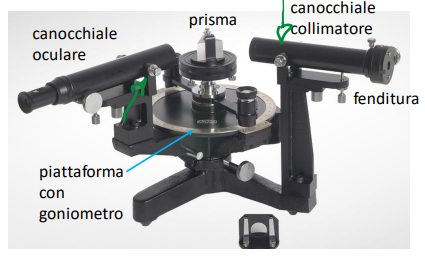
\includegraphics[width=0.55\linewidth]{Immagini ottica/apparato spettr..png}
    \caption{spettroscopio di Kirchhoff-Bunsen.}
    \label{fig: spettroscopio}
\end{figure}

Per determinare la posizione di deviazione minima, i passi da seguire sono:
\begin{enumerate}
    \item in assenza del prisma, si ruota il cannocchiale inquadrando la riga corrispondente alla fenditura. Poi si ripone il prisma sulla piattaforma e si seguono le righe spettrali fino a che queste non raggiungono la posizione di minimo. Questo accade quando si nota che le righe ``invertono il proprio moto'';
    \item si misurano le posizioni angolari di ciascuna riga dello spettro in questa condizione;
    \item l'angolo di deviazione $D_m$ è dato dalla differenza tra la posizione del raggio non deviato e quella delle righe, per cui $D_m=\ang{360}-\theta$;
    \item per calcolare le stime di $n$ si usa l'equazione \eqref{eq: indice rifrazione prisma dev. min.};
    \item ottenuti i valori di $n$ per le diverse lunghezze d'onda si opera una regressione di $n(\lambda)$ con la legge di Cauchy
    \begin{equation}
        n(\lambda)=A+\frac{B}{\lambda^2},\quad A,B\in\mathbb{R}.
    \end{equation}
\end{enumerate}
Per determinare l'indice di rifrazione del prima, i passi da seguire sono:
    \begin{enumerate}
        \item si sostituisce il prisma con il reticolo e si guarda nel cannocchiale dove si vedono $N$ spettri, uno per ogni ordine massimo, a destra e a sinistra della riga centrale (per ordini superiori a $m=2$ le righe di diversi ordini si possono sovrapporre);
        \item analogamente a quanto fatto con il prisma si misurano le posizioni angolari di alcune righe per gli ordini $m=1,2,3$;
        \item dalla formula $p\sin{\theta}=m\lambda$ si ricavano i valori di $\lambda$ di ogni riga misurata.
    \end{enumerate}
Per determinare lo spettro del mercurio, i passi da seguire sono:
    \begin{enumerate}
        \item si avvicina la fibra ottica alla lampada a vapori di mercurio e si osservano i picchi di lunghezza d'onda riportati dal software;
        \item si confrontano i valori dello spettrofotometro con quelli ricavati con lo spettroscopio.
    \end{enumerate}
\begin{obs}
    Il reticolo di diffrazione è un componente ottico costituito solitamente da una lastra di vetro sulla cui superficie è incisa una trama di linee parallele, uguali ed equidistanti, a distanze confrontabili con la lunghezza d'onda della luce. Sfrutta il principio ottico dell'interferenza di moltissimi fasci di luce che abbiano una precisa relazione di fase tra loro, ottenuti facendo passare la luce attraverso un gran numero di fenditure regolari. Se la sorgente è policromatica per ogni massimo si formeranno $N$ picchi, uno per ciascuna componente dello spettro. Quindi, si formeranno $M$ spettri, uno per ogni ordine di massimo.
\end{obs}

\section{Interferometro}
Le ipotesi consistono nel conoscere lo spostamento dello specchio tramite la vite micrometrica e il goniometro dell'interferometro, insieme allo spessore della lastra di vetro e alla misura della camera a vuoto della pompa. L'esperienza si articola in tre parti in cui si vuole: misurare la lunghezza d'onda del laser He-Ne, stimare l'indice di rifrazione della lastra di vetro; stimare l'indice di rifrazione dell'aria.
\begin{figure}[H]
    \centering
    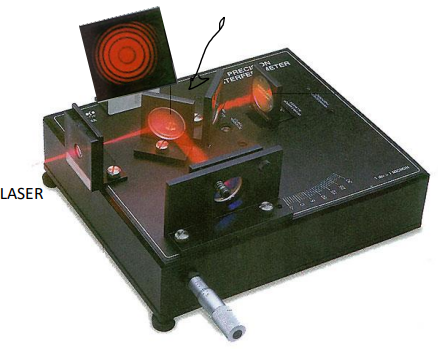
\includegraphics[width=0.5\linewidth]{Immagini ottica/interferometro.png}
    \caption{interferometro laser.}
    \label{fig: interferometro}
\end{figure}

\noindent
Per misurare la lunghezza d'onda del laser He-Ne, i passi da seguire sono:
\begin{enumerate}
    \item si varia la posizione dello specchio mobile e si contano le frange di interferenza che scompaiono (o appaiono, a seconda della direzione dello spostamento) nel centro della figura di interferenza; 
    \item si conta un numero $N$ fisso di frange (80 circa) e si registra lo spostamento $\Delta x$ indicato dalla vite micrometrica;
    \item ripetendo la misura $M$ volte, si ricava la lunghezza d'onda da
    \begin{equation}
        \lambda=\frac{2\Delta x}{N}.
    \end{equation}
\end{enumerate}
Per stimare l'indice di rifrazione della lastra di verto, i passi da seguire sono:
\begin{enumerate}
        \item si varia l'inclinazione della lastra rispetto al raggio incidente: il cambiamento di cammino ottico indotto dall'inclinazione fa muovere le frange di interferenza;
        \item di nuovo si conta un numero $N$ fisso di frange scomparse o apparse (50 circa) e si registra l'angolo $\theta$, misurato con un goniometro con precisione di un decimo di grado; 
        \item si ripete la misura $M$ volte e si ricava $n_{vetro}$ tramite la formula
        \begin{equation}
        n_{vetro}=\frac{(2t-N\lambda)(1-\cos{\theta})}{2t(1-\cos{\theta})-N\lambda},
    \end{equation}
    dove $t$ è lo spessore della lastra.
    \end{enumerate}
Per stimare l'indice di rifrazione dell'aria, i passi da seguire sono:
\begin{enumerate}
    \item si introduce su uno dei bracci dell'interferometro una camera, entro la quale è possibile variare la pressione usando una pompa a mano misurabile con un manometro con precisione di 100 mbar;
    \item Il manometro misura la differenza di pressione tra l'atmosfera e l'interno della camera. Un pulsante consente di far entrare o uscire lentamente l'aria dalla camera. Il procedimento consiste nel portare la camera ad un valore di $\Delta p$ desiderato;
    \item la variazione di pressione induce una variazione di indice di rifrazione, muovendo le frange di interferenza;
    \item si conta quante frange $N$ scompaiono (o appaiono) per una data variazione di pressione $\Delta p$. Si costruisce il grafico avente $\Delta p$ in ascisse e $N$ in ordinate;
    \item Conoscendo la lunghezza $d$ della camera a vuoto, si estrapola il valore del coefficiente angolare $m$ della retta e si calcola $n_{aria}$ dell'aria tramite la formula
    \begin{equation}
        n_{aria}=1+\frac{\lambda m}{2d}.
    \end{equation}
\end{enumerate}

\section{Polarimetro di Laurent}
L'esperienza si basa sull'utilizzo di sostanze otticamente attive e sul fenomeno consistente nella rotazione del piano di polarizzazione in uscita dalla soluzione contente tali sostanze, rispetto a quello in entrata. Inoltre, sfruttando il fenomeno della birifrangenza e il fatto che il vettore elettrico del raggio ordinario e straordinario vibrano in direzioni perpendicolari tra loro, è possibile ottenere un'onda polarizzata linearmente facendo in modo che uno dei fasci subisca riflessione totale. 

Le ipotesi dell'esperienza consistono nell'assumere che le misure si svolgono a temperatura costante e che la lampada al sodio sia una sorgente monocromatica. L'esperienza si articola quindi in due parti in cui si vuole stimare la concentrazione di fruttosio e saccarosio in alcune soluzioni acquose e verificare la legge di Malus tramite un filtro polarizzatore.
\begin{figure}[h]
    \centering
    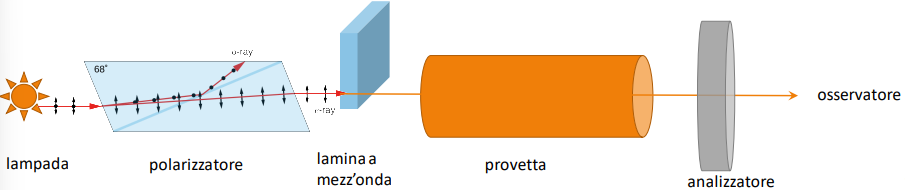
\includegraphics[width=0.9\linewidth]{Immagini ottica/polarizzatore.png}
    \caption{diagramma polarimetro di Laurent.}
    \label{fig: polarimetro}
\end{figure}

L'azione del polarimetro di Laurent si riassume in breve così: la luce generata dalla lampada al sodio viene polarizzata linearmente dal prisma di Nicol, metà di questo fascio attraversa una lamina a mezz'onda, mentre l'altra metà prosegue senza variazioni dello stato di polarizzazione; entrambi i fasci attraversano quindi un analizzatore. Ora, per determinare la concentrazione di saccarosio e fruttosio, i passi da seguire sono:
\begin{enumerate}
    \item si osserva che campi sono illuminati in modo diverso corrispondono all'effetto dell'analizzatore sui fasci;
    \item si ruota l'analizzatore fino a che i campi hanno la stessa illuminazione nella condizione di ``bassa illuminazione'' e si misura l'angolo $\theta$ al quale ciò avviene, una sola volta per il polarimetro scarico ($\theta'$), le altre volte con le provette di soluzione acquosa;
    \item sapendo che l'angolo $\alpha$ di rotazione del piano di polarizzazione è $\alpha=\theta-\theta'$ per il saccarosio, mentre $\alpha=(\theta-\theta')-\ang{180}$ per il fruttosio, si usa la legge di Biot
    \begin{equation}
        \label{eq: legge di biot}
        \alpha=kcl,
    \end{equation}
    dove $k$ è il potere rotatorio specifico della sostanza, $c$ è la concentrazione e $l$ è la lunghezza della provetta;
    \item noto $\alpha$ si stimano i valori di $c$ per diversi campioni.
\end{enumerate}
Per verificare la legge di Malus, i passi da seguire sono:
\begin{enumerate}
    \item si verifica che il fascio sia polarizzato linearmente controllando che siano visibili zeri di luce ruotando in polarizzatore di 360°. In caso contrario, si aggiunge un filtro polarizzante tra laser e analizzatore;
    \item si misura la corrente per ogni angolo, si graficano i dati e si effettua una regressione con la legge di Malus $I=I_0\cos^2{\theta}$.
\end{enumerate}

\section{Esperienza effetto fotoelettrico}
L'ipotesi dell'esperienza consiste solamente nel conoscere le lunghezze d'onda dei LED, mentre l'obiettivo di quest'ultima consiste nello stimare la constante di Planck $h$. Per farlo, i passi da seguire sono:
\begin{enumerate}
    \item si pone il LED all'interno della scatola scura in modo da evitare contaminazioni dalla radiazione di fondo;
    \item si applica il potenziale di controcampo e per ogni valore di questo si annota la fotocorrente prodotta dal LED tramite effetto fotoelettrico;
    \item si grafica la corrente in funzione della tensione e si determina il valore di tensione per cui la corrente si annulla;
    \item ottenuti questi particolari valori della corrente di controcampo per ogni LED, si mettono in un grafico in funzione della frequenza di ogni LED espressa in THz e si stima la costante di Planck calcolando il coefficiente angolare tramite una regressione lineare. 
\end{enumerate}
\begin{obs}
    La luce è emessa sotto forma di fotoni che si propagano alla velocità della luce $c$ e che hanno massa nulla. L'energia del fotone è data dalla relazione di Planck-Einstein $E=h\nu$. Nel processo fotoelettrico il fotone è completamente assorbito dall'elettrone. Questo per essere emesso deve acquistare un'energia minima pari a $W=h\nu_{lim}$, mentre non si ha alcuna emissione per $\nu<\nu_{lim}$. L'energia cinetica dell'elettrone quindi è $E_K=h\nu-\Delta E$, dove $\Delta E$ è l'energia persa dall'elettrone per allontanarsi dal metallo. Questa perdita è dovuta sia a possibili urti con le altre cariche presenti nel metallo, sia al superamento della funzione lavoro $W$. Il valore massimo dell'energia cinetica acquistata dall'elettrone emesso è 
    \begin{equation}
        E_{K,max}=h\nu-W.
    \end{equation}
    Queste ipotesi spiegano tutti i risultati sperimentali e introducono il primo esempio di dualismo onda-particella.
\end{obs}

\end{document}
